\chapter{Области на Скот}
\index{област на Скот}

В тази глава ще разгледаме понятията, които са ни нужни за дефинирането на понятието денотационна семантика на една програма.

\section{Частични наредби}
\index{частична наредба}

Бинарната релация $\sqsubseteq$ върху множеството $A$ се нарича {\bf частична наредба}, ако тя е:
\marginpar{На англ. \emph{partial order}}
\begin{itemize}
\item 
  рефлексивна, т.е. $(\forall a \in A)[a \sqsubseteq a]$;
\item
  транзитивна, т.е. $(\forall a,b,c \in A)[a \sqsubseteq b\ \&\ b \sqsubseteq c \implies a \sqsubseteq c]$;
\item
  антисиметрична, т.е. $(\forall a,b \in A)[a \sqsubseteq b\ \&\ b \sqsubseteq a  \implies a = b]$.
\end{itemize}
Една такава двойка $(A, \sqsubseteq)$ се нарича частично наредено множество.

\begin{example}
  Да означим 
  \[\F_n \df \{f:\Nat^n\to\Nat \mid f\text{ е частична функция}\}.\]
  \marginpar{Често вместо $x_1,\dots,x_n$ ще пишем просто $\ov{x}$.}
  Дефинираме и релацията {\bf включване } между две частични функции по следния начин:
  \begin{align*}
    f \subseteq g \dfff (\forall \ov{x}\in \Nat^n)[& f(\ov{x})\text{ не е деф.}\ \vee\\
                                            & (f(\ov{x})\text{ е деф.}\ \&\ g(\ov{x})\text{ е деф.}\ \&\ f(\ov{x}) = g(\ov{x}))].
  \end{align*}
  Да дефинираме също {\bf графиката} на частичната функция $f$ като
  \[\Graph{f} \df \{\pair{\ov{x},y} \mid f(\ov{x}) = y\}.\]
  Тогава лесно се съобразява, че 
  \[f \subseteq g \iff \Graph{f} \subseteq \Graph{g}.\]
  Съобразете, че двойката $(\Partial{\Nat}{\Nat}, \subseteq)$ е частично наредено множество.
\end{example}

\marginpar{Обърнете внимание, че има и понятие \emph{минимален} елемент, което в общия случай е различно от понятието \emph{най-малък} елемент. Един елемент $a_0$ е минимален за множеството $A$, ако $\neg(\exists a \in A)[a \sqsubseteq a_0\ \&\ a \neq a_0]$. Съобразете, че е възможно едно частично наредено множество да притежава повече от един минимални елементи.}
Казваме, че $a_0$ е {\bf най-малък елемент} на частично нареденото множество $(A, \sqsubseteq)$,
ако $(\forall a \in A)[a_0 \sqsubseteq a]$. Ако такъв елемент съществува, то той е единствен,
защото релацията $\sqsubseteq$ е антисиметрична.
% {\bf Неподвижна точка} на $f:A \to A$ е елемент $a \in A$, такъв че $f(a) = a$.
За по-кратко монотонно-растящите редици от елементи на $A$,
\[a_0 \sqsubseteq a_1 \sqsubseteq \cdots \sqsubseteq a_n \sqsubseteq \cdots,\]
ще наричаме (растящи) {\bf вериги}. 

Един елемент $b$ е {\bf горна граница} на веригата $\chain{a}{n}$, ако 
$(\forall n)[a_n \sqsubseteq b]$.
Един елемент $b$ е {\bf точна горна граница} на веригата $\chain{a}{n}$, ако са изпълнени свойствата:
\begin{itemize}
\item 
  $(\forall n)[a_n \sqsubseteq b]$, т.е. $b$ е горна граница;
\item
  за всяка друга горна граница $c$ е изпълнено, че $b \sqsubseteq c$, т.е.
  $b$ е най-малкият елемент измежду всички горни граници на веригата $\chain{a}{n}$.
\end{itemize}
Не всяка верига притежава точна горна граница.
Обикновено точната горна граница на вергата $\chain{a}{n}$ ще бележим като $\bigsqcup_n a_n$.

\Stefan{Още тук да се даде пример за верига от частични функции и две функции - една, която е точна горна граница на веригата и една, която е просто горна граница.}


\begin{framed}
  \begin{definition}
    Наредена тройка от вида $\A = (A, \sqsubseteq, \bot)$ се нарича {\bf област на Скот}, ако:
    \index{област на Скот}
    \begin{itemize}
    \item
      $\sqsubseteq$ е бинарна релация върху $A$, която задава частична наредба.
    \item
      Всяка растяща верига $\chain{a}{n}$ в $A$ притежава точна горна граница $\bigsqcup_n a_n$.
    \item
      $\bot \in A$ е най-малкият елемент на $A$;
    \end{itemize}
  \end{definition}
\end{framed}

\marginpar{На англ. {\em Scott domain}. Обикновено в литературата, за да се нарече едно частично нареденото множество област на Скот се изискват още допълнителни свойства, но за нашите цели тази дефиниция ще свърши работа.}

Интуицията зад израза $a \sqsubseteq b$ е, че $b$ носи повече информация от $a$, без да противоречи на $a$. Елементът $\bot$ означава липса на информация.

\begin{example}
  Тройката $\Partial{\Nat^n}{\Nat} \df (\ \F_n,\ \subseteq,\ \bm{\emptyset}^{(n)}\ )$ е област на Скот, където:
  \begin{itemize}
  \item
    С $\F_n$ означаваме всички частични функции от $\Nat^n$ в $\Nat$.
  \item
     релацията ,,включване'' между функции е дефинирана по следния начин:
     \[f\subseteq g\ \dffff\ \text{Graph}(f) \subseteq \text{Graph}(g).\]
   \item
     $\bm{\emptyset}^{(n)}$ е функцията с празна дефиниционна област, т.е. $\Dom(\bm{\emptyset}^{(n)}) = \emptyset$.
  \end{itemize}
\end{example}

\marginpar{В хаскел $\bot$ се означава като \vv{undefined}. Повече за денотационна семантика в хаскел може да прочетете \href{https://en.wikibooks.org/wiki/Haskell/Denotational_semantics}{тук}.}

\begin{example}
  Да разгледаме няколко примера, които вече сме срещали.
  \begin{itemize}
  \item
    $(\Ps(\Nat),\subseteq,\emptyset)$ е област на Скот.
  \item
    $(\Nat, \leq, 0)$ не е е област на Скот.
  \item
    $(\Nat\cup\{\infty\}, \leq, 0)$ е област на Скот, където наредбата $\leq$ е зададена като
    \[0 \leq 1 \leq \cdots \leq \infty.\]
  \item
    $(\{0,1\}^\star, \preceq, \varepsilon)$ не е област на Скот, където $\preceq$ е релацията префикс на две думи.
  \end{itemize}
\end{example}

\begin{example}
  Да разгледаме множеството 
  \[Bin^\infty = \{\sigma \mid \sigma :\{0,1,2,\dots,n-1\} \to \{0,1\}\ \&\ n \in \Nat\} \cup 
  \{f \mid f:\Nat \to \{0,1\}\}\]
  съставено от всички крайни и безкрайни двоични низове.
  \begin{itemize}
  \item
    Да разгледаме релацията
    \[\sigma \preceq \tau \iff \abs{\sigma} \leq \abs{\tau}\ \&\ (\forall i < |\sigma|)[\sigma(i) = \tau(i)],\]
    т.е. $\sigma$ е префикс на $\tau$.    
  \item
    Да означим с $\varepsilon$ единствения двоичен низ с дължина $0$. С други думи, $\varepsilon$ е празната функция.
  \end{itemize}
  Тогава $Bin^\infty = (Bin^\infty,\preceq,\varepsilon)$ е област на Скот.
\end{example}

\marginpar{Тези две свойства ще се окажат полезни по-нататък.}
\begin{problem}
  Нека $\chain{a}{i}$ и $\chain{b}{i}$ са вериги в областта на Скот $\A$, за които е изпълнено, че
  $a_i \sqsubseteq b_i$ за всяко $i$.
  Докажете, че $\bigsqcup_i a_i \sqsubseteq \bigsqcup_i b_i$.
\end{problem}

\begin{problem}
  Нека $\chain{a}{i}$ е верига в областта на Скот $\A$ и нека $k$ е естествено число.
  Докажете, че $\bigsqcup_i a_i = \bigsqcup_i a_{i+k}$.
\end{problem}

\begin{problem}
  \marginpar{Езикът $\{a^nb^n\mid n\in\Nat\}$ може да се представи като обединение на безкрайна верига от крайни езици.}
  Нека $\Sigma$ е азбука. Да разгледаме тройката $\mathcal{R} = (Reg, \subseteq, \emptyset)$, където $Reg$ е съвкупността от всички регулярни езици над $\Sigma$.
  Вярно ли е, че $\mathcal{R}$ е област на Скот ?
\end{problem}

\begin{problem}
  Нека $\mathcal{P} = (P, \preceq)$ да бъде частична наредба.
  Да дефинираме частичната наредба $\mathcal{C} = (\texttt{Chain}(P), \sqsubseteq)$, където:
  \begin{itemize}
  \item
    $\texttt{Chain}(P) = \{\ov{x} \mid \ov{x} = \chain{x}{i} \text{ е верига в }P\}$;
  \item
    $\ov{x} \sqsubseteq \ov{x}' \iff (\forall i)[\ x_i \preceq x'_i\ ]$ 
  \end{itemize}
  Докажете, че ако $\mathcal{P}$ формира област на Скот, то
  $\mathcal{C}$ също формира област на Скот.
\end{problem}



%%% Local Variables:
%%% mode: latex
%%% TeX-master: "../sep"
%%% End:


\section{Конструкции}

Ще разгледаме няколко конструкции, с които ще видим как можем да строим по-сложни области на Скот.

\subsection{Плоска област на Скот}

\Stefan{По принцип плоската област на Скот се дефинира върху друга област на Скот.}

Ще започнем с една проста конструкция, чрез която можем да разширим всяко множество до област на Скот по един почти тривиален начин.

Да фиксираме едно произволно непразно множество $A$ и един елемент $\bot \not \in A$.
Да означим $A_\bot = A \cup \{\bot\}$ и да разгледаме следната бинарна релация $\sqsubseteq$ върху $A_\bot$:
\[a \sqsubseteq b\ \iff\ a = \bot\ \vee\ a = b.\]
Лесно се съобразява, че $\sqsubseteq$ задава {\em частична наредба} върху $A_\bot$:
\marginpar{От деф. на $\sqsubseteq$ следва, че $\bot$ е най-малкият елемент}
\begin{itemize}
\item 
  {\em рефлексивност}: $a \sqsubseteq a$ за всяка $a \in A_\bot$;
\item
  {\em транзитивност}: $a \sqsubseteq b\ \&\ b \sqsubseteq c \implies a\sqsubseteq c$ за всеки $a,b,c \in A_\bot$;
\item
  {\em антисиметричност}: $a \sqsubseteq b\ \&\ b\sqsubseteq a \implies a = b$ за всеки $a,b \in A_\bot$.
\end{itemize}

Наредбата $(A_\bot, \sqsubseteq)$ ще наричаме {\bf плоска наредба}. Тя ще играе важна роля в нашите разглеждания.
\marginpar{$\bot$ се нарича {\em bottom} елемент}
Например, често ще разглеждаме плоската наредба $(\Nat_\bot, \sqsubseteq)$.

\begin{framed}
  \begin{figure}[H]
    \label{fig:flat-nat-1}
    \centering
    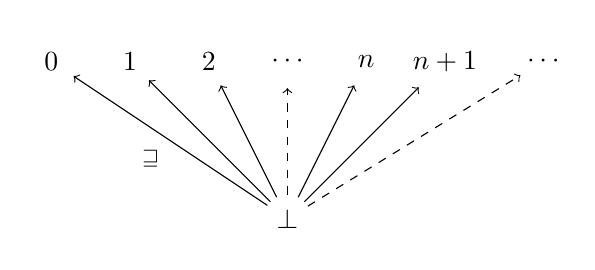
\begin{tikzpicture}[shorten >=1pt,->]
      \tikzstyle{vertex}=[circle,minimum size=17pt,inner sep=0pt]
      
      \node[vertex] (bot) at (3,0) {$\bot$};
      \node[vertex] (0) at (0,2) {$0$};
      \node[vertex] (1) at (1,2) {$1$};
      \node[vertex] (2) at (2,2) {$2$};
      \node[vertex] (dots) at (3,2) {$\cdots$};
      \node[vertex] (n) at (4,2) {$n$};
      \node[vertex] (n1) at (5,2) {$n+1$};
      \node[vertex] (ddots) at (6.25,2) {$\cdots$};
      
      \draw (bot) -- node[below left]{$\scriptstyle{\sqsupseteq}$} (0);
      \draw (bot) -- (1);
      \draw (bot) -- (2);
      \draw[dashed] (bot) -- (dots);
      \draw (bot) -- (n);
      \draw (bot) -- (n1);
      \draw[dashed] (bot) -- (ddots);
    \end{tikzpicture}    
    \caption{Графично представяне на плоската наредба $\sqsubseteq$ върху $\Nat_\bot$}
  \end{figure}
  \end{framed}

\begin{proposition}
  \index{област на Скот!плоска}
  Нека $A$ е произволно множество и нека елементът $\bot \not \in A$.
  \marginpar{На англ. {\em flat domain}}
  Определяме наредената тройка $\A_\bot = (A_\bot, \sqsubseteq, \bot)$ като:
  \begin{itemize}
  \item 
    $A_\bot = A\cup\{\bot\}$;
  \item
    $\sqsubseteq$ задава {\em плоската наредба} върху $A_\bot$.
  \end{itemize}
  Тогава $\A_\bot$ е област на Скот, която ще наричаме {\bf плоска област на Скот} за множеството $A$.
\end{proposition}

%%% Local Variables:
%%% mode: latex
%%% TeX-master: "../sep"
%%% End:


\subsection{Крайно произведение}
\label{subsect:domains:product}
\index{област на Скот!крайно произведение}
\marginpar{Това е една от най-простите конструкции върху области на Скот. Вижте например \cite[стр. 125]{winskel} и \cite[176]{models-of-computation}.}

Нека $\A$ и $\B$ са области на Скот.
Тогава $\A \times \B \df (A \times B,\sqsubseteq,\bot)$, където
\begin{itemize}
\item
  $A \times B = \{\pair{a,b} \mid a \in A\ \&\ b \in B\}$;
\item
  $\pair{a,b} \sqsubseteq \pair{a',b'} \iff a \sqsubseteq^\A a'\ \&\ b \sqsubseteq^\B b'$;
\item
  $\bot = \pair{\bot^\A,\bot^\B}$.
\end{itemize}

\begin{framed}
  \begin{proposition}
    \label{pr:cartesian}
    Ако $\A$ и $\B$ са области на Скот, то $\A \times \B$ е област на Скот.
  \end{proposition}  
\end{framed}
\begin{hint}
  Лесно се съобразява, че $\sqsubseteq$ е частична наредба и че $\bot$ е най-малкият елемент.
  Да разгледаме една верига $\{\pair{a_i,b_i}\}^\infty_{i=1}$ в $\A \times \B$.
  Лесно се вижда, че
  \[\bigsqcup_i\pair{a_i,b_i} = \pair{\bigsqcup_ia_i,\bigsqcup_ib_i}.\]
  \begin{itemize}
  \item
    За произволен елемент $\pair{a_i,b_i}$ от веригата е ясно, че $a_i \sqsubseteq^\A \bigsqcup_ia_i$ и $b_i \sqsubseteq^\B \bigsqcup_i b_i$.
    Следователно, $\pair{\bigsqcup_ia_i,\bigsqcup_ib_i}$ е горна граница на веригата.
  \item
    Нека $\pair{c,d}$ е горна граница на веригата, т.е. за всяко $i$,
    $a_i \sqsubseteq^\A c$ и $b_i \sqsubseteq^\B d$.
    Но тогава $c$ е горна граница на веригата $\chain{a}{i}$ и следователно $\bigsqcup_ia_i \sqsubseteq^\A c$.
    Също така, $d$ е горна граница на веригата $\chain{b}{i}$ и следователно $\bigsqcup_i b_i \sqsubseteq^\B d$.
    Заключаваме, че $\pair{\bigsqcup_ia_i,\bigsqcup_ib_i} \sqsubseteq \pair{c,d}$, т.е. $\pair{\bigsqcup_ia_i,\bigsqcup_ib_i}$
    е точна горна граница на веригата.
  \end{itemize}
\end{hint}

Нека $\A_1,\dots,\A_n$, $n \geq 2$, са области на Скот. Дефинираме 
$\prod^n_{i=1}\A_i = (A, \sqsubseteq, \bot)$ по следния начин:
\begin{itemize}
\item
  Ако $n = 2$, то $\prod^2_{i=1} \A_i \df \A_1 \times \A_2$.
\item
  Ако $n > 2$, то $\prod^n_{i=1} \A_i \df (\prod^{n-1}_{i=1}\A_i) \times \A_n$.
\end{itemize}

Използвайки \Prop{cartesian}, лесно се съобразява следното твърдение.
\begin{proposition}
  Ако $\A_1,\dots,\A_n$, $n \geq 2$, са области на Скот, то $\prod^n_{i=1}\A_i$ е област на Скот.
\end{proposition}

\begin{framed}
  \begin{figure}[H]
    \centering
    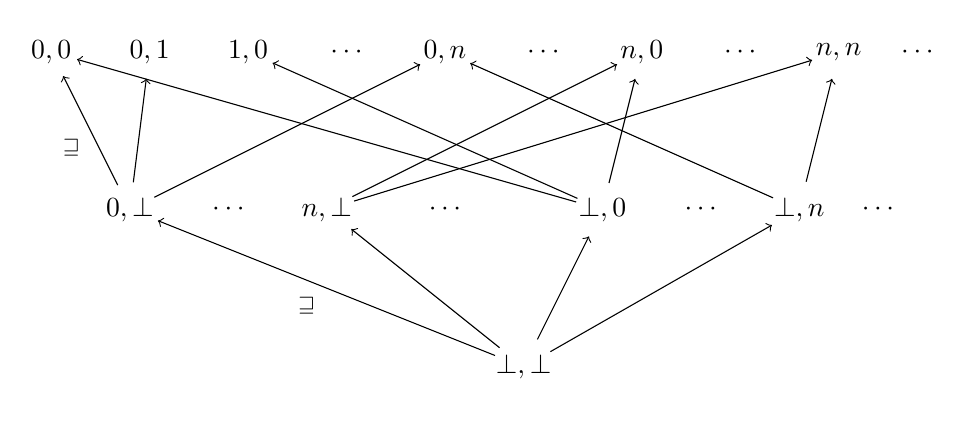
\begin{tikzpicture}[shorten >=1pt,->]
      \tikzstyle{vertex}=[circle,minimum size=17pt,inner sep=0pt]
      
      \node[vertex] (bot) at (5,-1) {$\pair{\bot,\bot}$};
      
      \node[vertex] (0b) at (0,1) {$\pair{0,\bot}$};
      \node[vertex] (db) at (1.25,1) {$\cdots$};
      \node[vertex] (nb) at (2.5,1) {$\pair{n,\bot}$};
      \node[vertex] (ddb) at (4,1) {$\cdots$};
      
      \node[vertex] (b0) at (6,1) {$\pair{\bot,0}$};
      \node[vertex] (bd) at (7.25,1) {$\cdots$};
      \node[vertex] (bn) at (8.5,1) {$\pair{\bot,n}$};
      \node[vertex] (bdd) at (9.5,1) {$\cdots$};
      
      \node[vertex] (00) at (-1,3) {$\pair{0,0}$};
      \node[vertex] (01) at (0.25,3) {$\pair{0,1}$};
      \node[vertex] (10) at (1.5,3) {$\pair{1,0}$};
      \node[vertex] (ddd) at (2.75,3) {$\cdots$};
      \node[vertex] (0n) at (4,3) {$\pair{0,n}$};
      \node[vertex] (dddd) at (5.25,3) {$\cdots$};
      \node[vertex] (n0) at (6.5,3) {$\pair{n,0}$};
      \node[vertex] (ddddd) at (7.75,3) {$\cdots$};
      \node[vertex] (nn) at (9,3) {$\pair{n,n}$};
      \node[vertex] (dddddd) at (10,3) {$\cdots$};

      \draw (bot) -- node[below left]{$\scriptstyle{\sqsupseteq}$} (0b);
      \draw (bot) -- (nb);
      \draw (bot) -- (b0);
      \draw (bot) -- (bn);

      \draw (0b) -- node[below left]{$\scriptstyle{\sqsupseteq}$} (00);
      \draw (0b) -- (01);
      \draw (0b) -- (0n);

      \draw (b0) -- (00);
      \draw (b0) -- (10);
      \draw (b0) -- (n0);
      \draw (nb) -- (n0);
      
      \draw (nb) -- (nn);
      \draw (bn) -- (0n);
      \draw (bn) -- (nn);

    \end{tikzpicture}    
    \caption{Графично представяне на част от $\sqsubseteq$ върху $\Nat^2_\bot$}
    \label{fig:flat-nat-2}
  \end{figure}
\end{framed}

Вижда се от \Figure{flat-nat-2}, че всяка верига в $\Nat^2_\bot$ има дължина най-много $3$.
Лесно се съобразява, че всяка верига в $\Nat^k_\bot$ има дължина най-много $k+1$.
Свойството, че всяка верига в $\Nat^k_\bot$ има само краен брой различни члена
ще се окаже важно по-нататък. Сега ще въведем понятие, което описва това свойство в произволна област на Скот.
\marginpar{ $\Nat^k_\bot \df \underbrace{\Nat_\bot \times \cdots \times\Nat_\bot}_{k}$. Какво става, когато $k = 0$ ? Това ще бъде важно по-нататък.}

Нека $\A$ е област на Скот и да разгледаме една верига $\chain{a}{n}$ в $\A$.
Ще казваме, че $\chain{a}{n}$ се {\bf стабилизира}, ако съществува индекс $n_0$, за който
\[(\forall n \geq n_0)[a_{n_0} = a_{n}],\]
т.е.
\[a_0 \sqsubseteq a_1 \sqsubseteq a_2 \sqsubseteq \cdots \sqsubseteq a_{n_0} = a_{n_0+1} = a_{n_0+2} = \cdots\]
От казаното по-горе следва, че всяка растяща верига в $\Nat^k_\bot$ се стабилизира.

\marginpar{Едни от основните области на Скот, които ще разглеждаме при дефинирането на денотационната семантика ще бъдат $\Nat_\bot$ и $\Nat^k_\bot$.}


% Добре е още тук да отбележим, че конструкцията за декартово произведение, която разглеждаме тук е опростен вариант на това, което имаме в хаскел.
% Да разгледаме един пример.
% \begin{haskellcode}
% ghci> :set +m -- multiline definitions
% ghci> let
%  | h :: (a,a) -> Int
%  | h _ = 4
%  | 
% ghci> h (2,3)
% 4
% ghci> h (2,undefined)
% 4
% ghci> h (undefined,undefined)
% 4
% ghci> h undefined
% 4
% ghci> 
% \end{haskellcode}

% Това означава, че ако искаме да моделираме по-точно декартово произведение на типове в хаскел чрез области на Скот, то би трябвало в областта на Скот $\A \times \B$
% да добавим \emph{нов} елемент $\bot^{\A\times\B}$, за който $\bot^{\A\times\B} \sqsubseteq (\bot^\A,\bot^\B)$.
% Ние не правим това, за да си улесним живота.

%%% Local Variables:
%%% mode: latex
%%% TeX-master: "../sep"
%%% End:


\index{област на Скот!изображения}
Нека $\A_i = (A_i,\ \sqsubseteq_i,\ \bot_i)$, за $i = 1,2$, са области на Скот.
Ще въведем няколко основни видове изображения между $\A_1$ и $\A_2$, 
които ще използваме често. След това ще разгледаме свойства на тези изображения
и ще видим каква е връзката между тях.
\begin{itemize}
\item
  Всяка тотална функция от вида $f:A_1 \to A_2$ ще наричаме изображение между областите на Скот $\A_1$ и $\A_2$
  и ще записваме $f:\A_1 \to \A_2$.
  \marginpar{Тук $\bm{\bot}$ е различно от $\bot$, макар и трудно да се различават графически. Освен това, $\A$ е различно от $A$.}
  Да въведем означението 
  \[\Mapping{\A_1}{\A_2} \df (\{f \mid f:\A_1 \to \A_2\},\ \sqsubseteq,\ \bm{\bot}),\]
  \marginpar{\todo Сами проверете, че така дефинираната релация $\sqsubseteq$ задава частична наредба, при положение, че $\sqsubseteq_2$ е частична наредба.}
  където имаме следната релация между изображенията $f,g:\A_1 \to \A_2$:
  \[f \sqsubseteq g \dfff (\forall a \in \A_1)[f(a) \sqsubseteq_2 g(a)].\]
  Също така, изображението $\bm{\bot}:\A_1 \to \A_2$ е дефинирано като
  \[(\forall a \in \A_1)[\bm{\bot}(a) = \bot_2].\]
\end{itemize}

На хаскел можем да дефинираме изображението $\bm{\bot}$ по следния начин:
\begin{haskellcode}
ghci> let bottom _ = undefined
\end{haskellcode}

\begin{framed}
  \begin{theorem}
    \label{th:all-mappings-is-domain}
    $\Mapping{\A_1}{\A_2}$ е област на Скот.
  \end{theorem}  
\end{framed}
\begin{proof}
  Нетривиалната част в доказателството е да проверим, че всяка верига $(f_i)^{\infty}_{i=0}$ в $\Mapping{\A_1}{\A_2}$
  притежава точна горна граница.
  % \marginpar{За по-кратко пишем $\bar{a}$ вместо $a_1,\dots,a_n$}
  Да разгледаме изображението $h:\A_1 \to \A_2$, където:
  \begin{equation}
    \label{eq:9}
    h(a) \df \bigsqcup \{f_i(a) \mid i \in \Nat\}.
  \end{equation}
  Ще докажем, че $h$ е тази точна горна граница.
  \begin{itemize}
  \item
    \marginpar{Това задължително трябва да се провери,
      защото например множеството $\{\bot, 0, 3\}$ \emph{няма} точна горна граница относно плоската наредба в $\Nat_\bot$.}
    Първо, трябва да се убедим, че дефиницията на $h$ е ,,смислена'', т.е. $h$ е тотална функция.
    Трябва да докажем, че за всяко $a\in \A_1$, точната горна граница 
    \[\bigsqcup\{f_i(a) \mid i \in \Nat\}\] съществува.
    Да фиксираме произволен елемент $a \in \A_1$.
    Получаваме следната верига в $\A_2$:
    \[f_0(a) \sqsubseteq f_1(a) \sqsubseteq f_2(a) \sqsubseteq \cdots \]
    Понеже $\A_2$ е област на Скот, то тази верига притежава точна горна граница в $\A_2$,
    която означачаваме като $\bigsqcup\{f_i(a) \mid i \in \Nat\}$, а според нашата дефиниция,
    това е точно $h(a)$.
    Това означава, че $h$ е тотална функция.
  \item
    Дотук имаме, че $h \in \Mapping{\A_1}{\A_2}$.
    Лесно се съобразява, че $h$ е горна граница на веригата $\chain{f}{i}$, защото за всеки елемент $a \in \A_1$
    и произволен индекс $k$,
    \[f_k(a) \sqsubseteq \bigsqcup\{f_i(a) | i \in \Nat\} \df h(a).\]
  \item
    Сега остава да проверим, че $h$ е точна горна граница, т.е. $h$ е най-малката измежду всички горни граници на 
    веригата $\chain{f}{i}$.
    Нека $g$ е друга горна граница на $\chain{f}{i}$. Това означава, че за всеки индекс $i$,
    $f_i \sqsubseteq g$. Следователно, за фиксирано $a \in \A_1$,
    $g(a)$ е горна граница за веригата $(f_i(a))^{\infty}_{i=0}$.
    Тогава е ясно, че за разглеждания елемент $a$,
    \[h(a) \df \bigsqcup\{f_i(a) \mid i\in\Nat\} \sqsubseteq g(a).\]
    Понеже елементът $a$ е прозиволен, получаваме, че $h \sqsubseteq g$.
  \item
    Доказахме, че $h$ е горна граница и че $h$ е най-малката измежду всички горни граници.
    Заключваме, че $h$ е {\em точната горна граница} на веригата $\chain{f}{i}$.
    \marginpar{Получаваме, че \[(\bigsqcup_if_i)(a) = \bigsqcup_i\{f_i(a)\}.\] Добре е да свикнете с тези означения, защото по-нататък ще ги използваме често.}
    С други думи,
    \[h = \bigsqcup_i f_i.\]
  \end{itemize}
\end{proof}

Завършваме с един важен частен случай на горната теорема.
\begin{framed}
  \begin{corollary}
    $\Mapping{\Nat^n_\bot}{\Nat_\bot}$ е област на Скот.
  \end{corollary}
\end{framed}


%%% Local Variables:
%%% mode: latex
%%% TeX-master: "../sep"
%%% End:


\subsection{Монотонни изображения}

\index{изображение!монотонно}
Да разгледаме областите на Скот $\A_1 = (A_1,\ \sqsubseteq_1,\ \bot_1)$ и $\A_2 =(A_2,\ \sqsubseteq_2,\ \bot_2)$.
Едно изображение $f:\A_1\to \A_2$ се нарича {\bf монотонно}, ако
\[(\forall a,a'\in\A_1)[a \sqsubseteq_1 a' \implies f(a) \sqsubseteq_2 f(a')].\]
Да въведем означението
\[\Mon{\A_1}{\A_2} \df (\{f: \A_1 \to \A_2 \mid f\text{ е мон. изобр.}\},\ \sqsubseteq,\ \bm{\bot}).\]

\begin{framed}
  \begin{theorem}\label{th:monotone-is-domain}
    $\Mon{\A_1}{\A_2}$ е област на Скот.
  \end{theorem}  
\end{framed}
\begin{hint}
  Да фиксираме една верига $\chain{f}{i}$ в $\Mon{\A_1}{\A_2}$. Трябва да докажем, че тази верига притежава точна горна граница,
  която е монотонно изображение.
  Да разгледаме същото изображение $h:\A_1 \to \A_2$ както в доказателството на \Th{all-mappings-is-domain}, като
  \[h(a) \df \bigsqcup \{f_i(a) \mid i \in \Nat\}.\]
  Оттам знаем, че $h$ е точна горна граница на веригата. 
  Остава да докажем, че $h \in \Mon{\A_1}{\A_2}$.
  Нека $a \sqsubseteq b$. Тогава, за всеки индекс $k$, понеже $f_k$ са монотонни изображения, получаваме следното:
  \[f_k(a) \sqsubseteq f_k(b) \sqsubseteq \bigsqcup \{f_i(b) \mid i \in \Nat\} \df h(b).\]
  Това означава, че $h(b)$ е горна граница за веригата ${(f_i(a))}^{\infty}_{i=0}$.
  Заключаваме, че 
  \begin{align*}
    h(a) & \df \bigsqcup \{f_i(a) \mid i \in \Nat\}\\
         & \sqsubseteq \bigsqcup \{f_i(b) \mid i \in \Nat\} \df h(b).
  \end{align*}
\end{hint}

Оттук като частен случай получаваме следното полезно следствие.
\begin{framed}
  \begin{corollary}\label{cr:flat-monotone-is-domain}
    $\Mon{\Nat^n_\bot}{\Nat_\bot}$ е област на Скот.
  \end{corollary}
\end{framed}

Удобно е да имаме следващото свойство на монотонните изображения като отделно твърдение за да можем да
се позоваваме на него, когато имаме нужда от него по-късно.

\begin{proposition}\label{pr:monotone-chain}
  Нека $f \in \Mon{\A}{\B}$ и $\chain{a}{i}$ е верига от елементи на $\A$.
  Тогава
  \[\bigsqcup_i f(a_i) \sqsubseteq f(\bigsqcup_i a_i).\]
\end{proposition}
\begin{proof}
  Понеже $f$ е монотонно, то ${(f(a_i))}^{\infty}_{i=0}$ е верига от елементи на областта на Скот $\B$
  и тя има точна горна граница.
  Достатъчно е да докажем, че $f(\bigsqcup_i a_i)$ е горна граница на веригата ${(f(a_i))}^{\infty}_{i=0}$.
  Но това е лесно.
  Понеже за произволен индекс $k$, $a_k \sqsubseteq \bigsqcup_i a_i$ и $f$ е монотонно изображение, то веднага получаваме, че
  $f(a_k) \sqsubseteq f(\bigsqcup_i a_i)$.
  Заключаваме, че $\bigsqcup_k f(a_k) \sqsubseteq f(\bigsqcup_i a_i)$.
\end{proof}

%%% Local Variables:
%%% mode: latex
%%% TeX-master: "../sep"
%%% End:


\subsection{Непрекъснати изображения}\index{изображение!непрекъснато}

\marginpar{На англ. {\em continuous}}
Едно изображение $f:\A_1\to \A_2$ се нарича {\bf непрекъснато}, ако са изпълнени свойствата:
\begin{itemize}
\item
  $f$ е монотонно изображение;
\item
  при всеки избор на верига $\chain{a}{i}$ в $\A_1$, имаме равенството
  \marginpar{Понеже $\A_1$ е област на Скот знаем, че $\bigsqcup_i a_i \in \A_1$}
  \marginpar{Понеже $f$ е монотонно, то ${(f(a_i))}^{\infty}_{i=0}$ е верига.}
  \marginpar{$\bigsqcup_i f(a_i) \df \bigsqcup\{f(a_i) \mid i \in \Nat\}$}
  \[f(\bigsqcup_i a_i) = \bigsqcup \{f(a_i) \mid i \in \Nat\}.\]  
\end{itemize}
Да означим
\[\Cont{\A_1}{\A_2} \df (\{f: \A_1 \to \A_2 \mid f\text{ е непр. изобр.}\},\ \sqsubseteq,\ \bm{\bot}).\]

% \begin{framed}
%   \begin{prop}
%     \label{pr:continuous-is-monotone}
%     За произволни области на Скот $\A_1$ и $\A_2$, всяко непрекъснато изображение $f:\A_1 \to \A_2$ е монотонно, т.е.
%     \[\Cont{\A_1}{\A_2}\ \subseteq\ \Mon{\A_1}{\A_2}.\]
%   \end{prop}
% \end{framed}
% \begin{proof}
%   Нека $f \in \Cont{\A_1}{\A_2}$.
%   Да вземем два произволни елемента в $\A_1$, за които $a \sqsubseteq_1 b$.
%   Ще докажем, че $f(a) \sqsubseteq_2 f(b)$.
%   Да разгледаме веригата $\chain{a}{i}$ в $\A_1$, където:
%   \[\underbrace{a_0}_{a} \sqsubseteq \underbrace{a_1}_{b} = \underbrace{a_2}_{b} = \underbrace{a_3}_{b} = \cdots\]
%   Ясно е, че 
%   \[\bigsqcup\{a_i \mid i \in \Nat\} = \bigsqcup\{a,b\} = b.\]
%   Тогава от непрекъснатостта на $f$ имаме, че
%   \begin{align*}
%     f(a) & = f(a_0) & \comment{\text{защото }a_0 \df a}\\
%     & \sqsubseteq_2 \bigsqcup\{f(a_i) \mid i \in \Nat\} & \comment{\text{защото }f(a_0) \in \{f(a_i) \mid i\in\Nat\}}\\
%     & = f(\bigsqcup_i a_i) & \comment{\text{защото $f$ е непр.}}\\
%     & = f(\bigsqcup\{a,b,b,b,\dots\}) & \comment{\text{от избора на веригата }\chain{a}{i}}\\
%     & = f(b) & \comment{\text{защото }a \sqsubseteq_1 b}.
%   \end{align*}
%   Така получихме, че за произволни $a,b\in\A_1$, 
%   \[a \sqsubseteq_1 b \implies f(a) \sqsubseteq_2 f(b).\]
% \end{proof}

Ясно е, че всяко непрекъснато изображение е монотонно.
Ествено е да си зададем въпроса дали имаме и обратното включване.
Оказва се, че в общия случай не е вярно, че всяко монотонно изображение е непрекъснато.

\begin{proposition}\label{pr:continuous-mappings-not-monotone}  
  Съществува област на Скот $\A$, за която
  \[\Cont{\A}{\A} \subsetneqq \Mon{\A}{\A}.\]
\end{proposition}
\begin{hint}
  Нека $A = \{a_n \mid n \in \Nat\} \cup \{a_\omega, b\}$.
  Да разгледаме областта на Скот $\A = (A, \sqsubseteq, a_0)$, където 
  наредбата между елементите е следната:
  \[a_0 \sqsubseteq a_1 \sqsubseteq \cdots \sqsubseteq a_n \sqsubseteq \cdots \sqsubseteq a_\omega \sqsubseteq b. \]
  Нека $f(a_n) = a_{n+1}$, $f(a_{\omega}) = b$ и $f(b) = b$.
  Очевидно е, че $f$ е монотонно изображение.
  Лесно се вижда, че $f$ не е непрекъснато изображение, 
  защото
  \[f(\bigsqcup_n a_n) = f(a_\omega) = b,\]
  но 
  \[\bigsqcup_n f(a_n) = \bigsqcup_n a_{n+1} = a_\omega.\]
\end{hint}

Сега да видим един важен за нас случай, при който имаме и обратното включване.
\marginpar{В Раздел~\ref{subsect:domains:product} дефинирахме какво означава една верига $\chain{n}{a}$ да се стабилизира: съществува индекс $n_0$, за който \[(\forall n \geq n_0)[a_{n_0} = a_{n}].\]}

\begin{framed}
  \begin{proposition}\label{pr:stab-continuous}
    Ако всяка верига в $\A_1$ се {\em стабилизира}, то
    \[\Mon{\A_1}{\A_2} \subseteq \Cont{\A_1}{\A_2}.\]
  \end{proposition}
\end{framed}
\begin{hint}
  Да разгледаме една верига $\chain{a}{i}$ в $\A_1$ и $f \in \Mon{\A_1}{\A_2}$.
  Ще докажем, че \[f(\bigsqcup_i a_i) = \bigsqcup_i f(a_i).\]

  \begin{enumerate}[(1)]
  \item
    % \marginpar{Това включване е вярно за произволна област на Скот $\A_1$.}
    % Ясно е, че за всяко монотонно изображение $f$,
    % понеже $a_i \sqsubseteq \bigsqcup_i a_i$, то $f(a_i) \sqsubseteq f(\bigsqcup_i a_i)$.
    % Това означава, че $f(\bigsqcup_i a_i)$ е горна граница на веригата $(f(a_i))^\infty_{i=0}$ в $\A_2$
    % и следователно
    % \[\bigsqcup_i f(a_i) \sqsubseteq f(\bigsqcup_i a_i).\]
    От \Prop{monotone-chain} веднага получаваме, че
    \[\bigsqcup_i f(a_i) \sqsubseteq f(\bigsqcup_i a_i).\]
  \item
    За другата посока ще използваме свойството, че веригата $\chain{a}{i}$ се стабилизира.
    Нека $n_0$ е индекс, такъв че $(\forall k \geq n_0)[a_k = a_{n_0}]$.
    Това означава, че $\bigsqcup_i a_i = a_{n_0}$.
    Тогава
    \[f(\bigsqcup_i a_i) = f(a_{n_0}) \sqsubseteq \bigsqcup_i f(a_i).\]
  \end{enumerate}
  
  От $(1)$ и $(2)$ следва, че $f(\bigsqcup_i a_i) = \bigsqcup_i f(a_i)$.
\end{hint}

От Раздел~\ref{subsect:domains:product} знаем, че всяка верига в $\Nat^n_\bot$ се {\em стабилизира}, то
получаваме следното важно следствие.
\begin{framed}
\begin{corollary}\label{cr:monotone-is-continuous}
  $\Mon{\Nat^n_\bot}{\Nat_\bot} = \Cont{\Nat^n_\bot}{\Nat_\bot}$.
\end{corollary}  
\end{framed}

% От доказателството на (1) за \Prop{stab-continuous} можем да извлечем следното свойство,
% което ще ни бъде полезно по-нататък.
% \begin{proposition}\label{pr:monotone-chain}
%   За всяко изображение $f \in \Mon{\A}{\B}$ и всяка верига $\chain{a}{i}$, е изпълнено, че
%   \[\bigsqcup_i f(a_i) \sqsubseteq f(\bigsqcup_i a_i).\]
% \end{proposition}

Понеже от \Cor{flat-monotone-is-domain} имаме, че монотонните изображения образуват област на Скот, 
то директно получаваме следната важна теорема.

\begin{framed}
\begin{theorem}
  \label{th:continuous-is-domain}
  $\Cont{\Nat^n_\bot}{\Nat_\bot}$ е област на Скот.
\end{theorem}
\end{framed}
% \begin{proof}
%   От \Cor{monotone-is-continuous} имаме, че 
%   \[\Mon{\Nat^n_\bot}{\Nat_\bot} = \Cont{\Nat^n_\bot}{\Nat_\bot}.\]
%   От \Cor{flat-monotone-is-domain} имаме, че 
%   \[(\Mon{\Nat^n_\bot}{\Nat_\bot}, \sqsubseteq, \Omega^{(n)})\]
%   е област на Скот. 
%   Оттук директно получаваме, че 
%   \[(\Cont{\Nat^n_\bot}{\Nat_\bot}, \sqsubseteq, \Omega^{(n)})\] е област на Скот.
% \end{proof}


% \begin{prop}
%   \label{pr:composition}
%   \index{изображения!композиция}
%   Ако $f \in \Cont{\A}{B}$ и $g \in \Cont{\B}{\C}$, то $g \circ f \in \Cont{\A}{\C}$,
%   където \[(g\circ f)(a) \df g(f(a)).\]
% \end{prop}
% \begin{hint}
%   Нека $\chain{a}{i}$ е верига в $\A$.
%   Да обърнем внимание, че понеже $f \in \Cont{\A}{\B}$,
%   то $f$ е монотонно изображение и тогава $(f(a_i))^\infty_{i=0}$ е верига в $\B$.
%   Тогава:
%   \begin{align*}
%     (g \circ f)(\bigsqcup_i a_i) & = g(f(\bigsqcup_i a_i)) & \comment{\text{от деф.}}\\
%     & = g(\bigsqcup_i f(a_i)) & \comment{f \text{ е непр.}}\\
%     & = \bigsqcup_i g(f(a_i)) & \comment{g \text{ е непр.}}
%   \end{align*}
% \end{hint}


\begin{problem}
  \marginpar{\cite[стр. 124]{reynolds}}
  Нека $f \in \Mon{\A}{\B}$ и $g \in \Mon{\B}{\A}$ имат свойствата:
  \begin{itemize}
  \item 
    $f\circ g = id_\B$;
  \item
    $g \circ f = id_\A$.
  \end{itemize}
  Докажете, че $f$ и $g$ са непрекъснати.
\end{problem}


% \begin{problem}
%   Нека $f_0 \sqsubseteq f_1 \sqsubseteq f_2 \sqsubseteq \cdots$
%   е верига от елементи на $\Cont{\A}{\A}$.
%   Да положим $h = \bigsqcup_n f_n$.
%   Вярно ли е, че 
%   \[h \circ h = \bigsqcup_n (f_n \circ f_n)?\]
%   Обосновете се!
% \end{problem}


\marginpar{Много от задачите са от \cite[стр. 31]{abramsky94}}

\begin{problem}
  Да разгледаме непрекъснатите изображения
  \[\Gamma,\Delta \in \Cont{\Cont{\A}{\A}}{\Cont{\A}{\A}}.\]
  \marginpar{Знаем, че изображението $\Gamma \circ \Delta$ е непрекъснато, където
    \[(\Gamma\circ\Delta)(f) \df \Gamma(\Delta(f)).\]}
  Винаги ли е вярно, че 
  \[\lfp(\Gamma \circ \Delta) \sqsubseteq \lfp(\Gamma) \circ \lfp(\Delta)?\]
  Обосновете се!
\end{problem}
% \ifhints
\begin{hint}
  Ще дадем контрапример.
  Нека $\A = \Nat_\bot$.
  Нека например да разгледаме
  \begin{align*}
    & \Delta(f)(x) \df f(x+1)\\
    & \Gamma(f)(x) \df
      \begin{cases}
        0, & x \neq \bot\\
        \bot, & x = \bot.
      \end{cases}
  \end{align*}
  Да положим $f_\Gamma \df \lfp(\Gamma)$ и $f_\Delta \df \lfp(\Delta)$.
  Ясно е, че 
  \begin{align*}
    & f_\Delta(x) = \bot\\
    & f_\Gamma(x) =
    \begin{cases}
      0, & x \neq \bot\\
      \bot, & x = \bot.
    \end{cases}  
  \end{align*}
  Тогава за произволно $x \in \Nat_\bot$,
  \[(f_\Gamma\circ f_\Delta)(x) = f_\Gamma(f_\Delta(x)) = f_\Gamma(\bot)  = \bot.\]
  От друга страна, понеже $(\Gamma \circ \Delta)(f) = \Gamma(\Delta(f))$, то 
  \begin{align*}
    & (\Gamma \circ \Delta)(f)(x) = \Gamma(\Delta(f))(x) = 
      \begin{cases}
        0, & x \neq \bot\\
        \bot, & x = \bot.
      \end{cases}
  \end{align*}
  Лесно се съобразява, че 
  \[\lfp(\Gamma \circ \Delta)(x) =
  \begin{cases}
    0, & x \neq \bot\\
    \bot, & x = \bot.
  \end{cases}\]
  Заключаваме, че 
  \[\lfp(\Gamma \circ \Delta) \sqsupset \lfp(\Gamma) \circ \lfp(\Delta).\]
\end{hint}
% \fi


\begin{problem}
  Да разгледаме операторите \[\Gamma,\Delta \in \Cont{\Cont{\A}{\A}}{\Cont{\A}{\A}}.\]
  Знаем, че операторът $\Gamma \circ \Delta$ е непрекъснат, където
  \[(\Gamma\circ\Delta)(f) \df \Gamma(\Delta(f)).\]
  Винаги ли е вярно, че:
  \[\lfp(\Gamma \circ \Delta) \sqsupseteq \lfp(\Gamma) \circ \lfp(\Delta)?\]
  Обосновете се!
\end{problem}
% \ifhints
\begin{hint}
  Ще дадем контрапример.
  Нека $\A = \Nat_\bot$.
  Нека например да разгледаме
  \begin{align*}
    & \Delta(f)(x) \df 0\\
    & \Gamma(f)(x) \df
      \begin{cases}
        0, & x = 0\\
        \bot, & \text{ иначе}.
      \end{cases}
  \end{align*}
  Да положим $f_\Gamma \df \lfp(\Gamma)$ и $f_\Delta \df \lfp(\Delta)$.
  Ясно е, че 
  \begin{align*}
    & f_\Delta(x) = 0\\
    & f_\Gamma(x) =
    \begin{cases}
      0, & x = 0\\
      \bot, & \text{ иначе}.
    \end{cases}  
  \end{align*}
  Тогава за произволно $x \in \Nat_\bot$,
  \[(f_\Gamma\circ f_\Delta)(x) = f_\Gamma(f_\Delta(x)) = f_\Gamma(0)  = 0.\]
  От друга страна, понеже $(\Gamma \circ \Delta)(f) = \Gamma(\Delta(f))$, то 
  \begin{align*}
    & (\Gamma \circ \Delta)(f)(x) = \Gamma(\Delta(f))(x) = 
      \begin{cases}
        0, & x = 0\\
        \bot, & \text{ иначе}.
      \end{cases}
  \end{align*}
  Лесно се съобразява, че 
  \[\lfp(\Gamma \circ \Delta)(x) =
  \begin{cases}
    0, & x = 0\\
    \bot, & \text{ иначе}.
  \end{cases}\]
  Заключаваме, че 
  \[\lfp(\Gamma \circ \Delta) \sqsubset \lfp(\Gamma) \circ \lfp(\Delta).\]
\end{hint}
% \fi


%%% Local Variables:
%%% mode: latex
%%% TeX-master: "../sep"
%%% End:


% \subsection{Точни изображения}

\marginpar{На англ. се нарича {\em strict}. ,,Стандартната'' семантика на хаскел е {\em non-strict}}
\index{изображение!точно}
Едно изображение $f:\A^n_1 \to \A_2$ се нарича {\bf точно}, ако 
\[(\forall \bar{a}\in\A^n_1)[\bot_1\in\{a_1,\dots,a_n\} \implies f(a_1,\dots,a_n) = \bot_2].\]
% Тук ще разглеждаме съвкупността от точни изображения:
% \[S_n \dff \{f: \Nat^n_\bot \to \Nat_\bot \mid f\text{ е точна}\}.\]
За произволни области на Скот $\A_1$ и $\A_2$, ще означаваме съвкупността от
точните изображения като $\Strict{\A_1}{\A_2}$.

\begin{example}
  Да разгледаме свойствата на няколко прости изображения.
  \begin{itemize}
  \item 
    Изображението $f:\Nat_\bot \to \Nat_\bot$, дефинирано като 
    \[f(x) = 42,\]
    за всяко $x \in \Nat_\bot$,
    {\bf не е точно}, защото $f(\bot) = 42$. Лесно се вижда, че $f$ е монотонно и непрекъснато изображение.
  \item
    От друга страна, изображението $g:\Nat_\bot \to \Nat_\bot$, дефинирано като 
    \[g(x) = \bot,\]
    за всяко $x \in \Nat_\bot$, {\bf е точно}, защото $g(\bot) = \bot$.
    Освен това, $g$ е монотонно и непрекъснато изображение.
  \end{itemize}
\end{example}

Видяхме, че лесно се намират монотонни изображения, които не са точни.
Сега ще разгледаме обратната посока.

\begin{proposition}
  \label{pr:strict-is-monotone}
  Всяко точно изображение $f:\Nat^n_\bot \to \Nat_\bot$ е също така и монотонно.
  С други думи, 
  \[\Strict{\Nat^n_\bot}{\Nat_\bot} \subseteq \Mon{\Nat^n_\bot}{\Nat_\bot}.\]
\end{proposition}
\begin{proof}
  Нека $f$ е точно и $\bar{a} \sqsubseteq \bar{b}$.
  Ще проверим, че 
  \[f(\bar{a}) = c \sqsubseteq d = f(\bar{b}).\]
  \begin{itemize}
  \item 
    Ако $c = \bot$, то е очевидно, че $c \sqsubseteq d$.
  \item
    Интересният случай е когато $c \neq \bot$. Тогава трябва да видим, че $c = d$.
    Понеже $f$ е точна и $c \neq \bot$, това означава, че $\bot \not\in\{a_1,\dots,a_n\}$.
    Но понеже $\sqsubseteq$ е плоска наредба, и $\bar{a} \sqsubseteq \bar{b}$, това означава, че $\bar{a} = \bar{b}$.
    Следотвателно, наистина $c = d$.
  \end{itemize}
\end{proof}

\begin{framed}
  \begin{theorem}
    \label{th:strict-is-domain}
    $(\Strict{\Nat^n_\bot}{\Nat_\bot},\ \sqsubseteq,\ \bm{\bot}^{(n)})$ е област на Скот.
  \end{theorem}
\end{framed}
\begin{hint}
  Да разгледаме веригата $\chain{f}{i}$ от елементи на $\Strict{\Nat^n_\bot}{\Nat_\bot}$.
  Трябва да докажем, че тази верига притежава точна горна граница, която също е точно изображение.
  % Понеже от \Prop{strict-is-monotone} имаме, че всяка точна функция е монотонна, то наготово от 
  От доказателството на \Th{all-mappings-is-domain} знаем, че изображението $h$ дефинирано за всяко $\bar{a} \in \Nat^n_\bot$ като
  \[h(\bar{a}) \df \bigsqcup \{f_i(\bar{a}) \mid i \in \Nat\}\]
  е точна горна граница на веригата $\chain{f}{i}$.
  Остава да проверим, че $h$ е точно изображение.
  Нека $\bar{a} \in \Nat^n_\bot$ и да приемем, че $\bot \in \{a_1,\dots,a_n\}$.
  Тогава:
  \begin{align*}
    h(\bar{a}) & = \bigsqcup \{f_i(\bar{a}) \mid i \in \Nat\} & \comment{\text{от деф. на }h}\\
               & = \bigsqcup\{\bot,\bot,\dots,\bot,\dots\} & \comment{f_i\text{ са точни}}\\
               & = \bot.
  \end{align*}
\end{hint}

\begin{example}
  \label{ex:simple-non-continuous}
  Нека сега да разгледаме $h:\Nat_\bot \to \Nat_\bot$, където 
  \begin{align*}
    h(x) = &
    \begin{cases}
      0, & \text{ако }x = \bot,\\
      1, & \text{иначе}.
    \end{cases}
  \end{align*}
  Да видим колко ,,лошо'' изображение е $h$:
  \begin{itemize}
  \item 
    $h$ не е точно, защото $h(\bot) \neq \bot$;
  \item
    $h$ не е монотонно, защото $\bot \sqsubseteq 5$, но $h(\bot) = 0 \not\sqsubseteq 1 = h(5)$;
  \item
    $h$ не е непрекъснато, защото $\Cont{\Nat_\bot}{\Nat_\bot} = \Mon{\Nat_\bot}{\Nat_\bot}$.
  \end{itemize}
  Нека да видим, че хаскел не позволява такива ,,лоши'' функции:

  \begin{haskellcode}
ghci> let h(x) = if x == undefined then 0 else 1
ghci> h(5)
*** Exception: Prelude.undefined
ghci> h(undefined)
*** Exception: Prelude.undefined
  \end{haskellcode}
\end{example}

\begin{example}
  \label{ex:non-strict-monotone}
  Да разгледаме $f:\Nat^2_\bot \to \Nat_\bot$ дефинирано като \[f(x,y) = x.\]
  \begin{itemize}
  \item 
    $f$ не е точно, защото $f(0,\bot) = 0$.
  \item
    $f$ е монотонно, защото ако $\pair{x,y} \sqsubseteq \pair{x',y'}$, то $x \sqsubseteq x'$ и
    \[f(x,y) = x \sqsubseteq x' = f(x',y').\]
  \item
    $f$ е непрекъснато, защото от \Cor{monotone-is-continuous} знаем, че 
    $\Mon{\Nat^2_\bot}{\Nat_\bot} = \Cont{\Nat^2_\bot}{\Nat_\bot}$.
  \end{itemize}
\end{example}

Можем да обобщим всичко, което направихме дотук, със следната илюстрация на основните области на Скот, с които ще работим
в \Chapter{rec}.

\begin{framed}
    \begin{align*}
      \Strict{\Nat^n_\bot}{\Nat_\bot} & \subsetneqq \Mon{\Nat^n_\bot}{\Nat_\bot} & \comment{\text{от \Ex{non-strict-monotone} и \Prop{strict-is-monotone}}}\\
      & = \Cont{\Nat^n_\bot}{\Nat_\bot} & \comment{\text{от \Prop{continuous-is-monotone} и \Cor{monotone-is-continuous}}}\\
      & \subsetneqq \Mapping{\Nat^n_\bot}{\Nat_\bot} & \comment{\text{от \Ex{simple-non-continuous}}}.
    \end{align*}
\end{framed}

\begin{example}
  \label{ex:plus}
  Да разгледаме $f:\Nat^2_\bot \to \Nat_\bot$ дефинирана по следния начин:
  \[f(x,y) = 
  \begin{cases}
    \bot, & x = \bot\ \&\ y = \bot\\
    x, & x \neq \bot\ \&\ y = \bot\\
    y, & x = \bot\ \&\ y \neq \bot\\
    x+y, & x \neq \bot\ \&\ y \neq \bot.
  \end{cases}\]
  Изображението $f$ не е точно, защото например $f(\bot,0) \neq \bot$.
  $f$ не е монотонно изображение, защото $\pair{2,\bot} \sqsubseteq \pair{2,3}$, но $2 = f(2,\bot) \not\sqsubseteq f(2,3) = 5$.
  Също така, $f$ не е непрекъснато изображение, защото $\Mon{\Nat^2_\bot}{\Nat_\bot} = \Cont{\Nat^2_\bot}{\Nat_\bot}$.
\end{example}
% \begin{hint}
%   \begin{itemize}
%   \item 
%     $f$ не е точно изображение, защото например
%     $f(\bot,0) \neq \bot$.
%   \item
%     $f$ не е монотонно. Например,
%     \[\pair{\bot,0} \sqsubseteq \pair{1,0}\ \&\ f(\bot,0) = 0 \not\sqsubseteq 1 = f(1,0).\]    
%   \item
%     $f$ не е непрекъснато, защото $\Cont{\Nat^2_\bot}{\Nat_\bot} = \Mon{\Nat^2_\bot}{\Nat_\bot}$.
%   \end{itemize}    
% \end{hint}


% \subsection{Точни продължения}
% \index{изображение!точно продължение}

% Нека $A$ и $B$ са произволни множества, а $\A_\bot$ и $\B_\bot$ са плоските области на Скот получени съответно от $A$ и $B$.
% За еднa частична функция $f:A^n \to B$, определяме точното изображение $f^\star:\A^n_\bot \to \B_\bot$ по следния начин:
% \marginpar{$f^\star \in \Strict{\A^n_\bot}{\B_\bot}$}
% \begin{align*}
%   f^\star(\ov{a}) \dff
%   \begin{cases}
%     f(\ov{a}), & \text{ако }\bot\not\in\{a_1,\dots,a_n\}\ \&\ f(\ov{a})\text{ е деф.}\\
%     \bot, & \text{иначе}.
%   \end{cases}
% \end{align*}
% Изображението $f^\star$ се нарича {\bf точно продължение} на $f$.

% \begin{example}
%   Да разгледаме частичната функция $f:\Nat^2 \to \Nat$, дефинирана като
%   $f(x,y) = x+y$. Тогава точното продължение на $f$ е 
%   \[f^\star(x,y) = 
%   \begin{cases}
%     x+y, & x,y\in\Nat\\
%     \bot, & x = \bot \vee y = \bot.
%   \end{cases}\]
% \end{example}

% \Stefan{За какво ми е точното продължение да е непрекъснато?}
% \noindent Да дефинираме оператор $\Sigma^\star : \Partial{\Nat^n}{\Nat} \to \Strict{\Nat^n_\bot}{\Nat_\bot}$ като
% \[\Sigma^\star(f) = f^\star.\] 
% Ще наричаме $\Sigma^\star$ {\bf продължаващ} оператор, защото на всяка частична функция дава нейното точно продължение.

% \begin{framed}
%   \begin{prop}
%     $\Sigma^\star$ е непрекъснато изображение, т.е.
%     \[\Sigma^\star \in \Cont{\Partial{\Nat^n}{\Nat}}{\Strict{\Nat^n_\bot}{\Nat_\bot}}.\]
%   \end{prop}
% \end{framed}
% \begin{hint}
%   Трябва да докажем, че за произволна верига $(f_i)^{\infty}_{i=0}$ от частични функции, 
%   $\Sigma^\star(\bigcup_i f_i) = \bigsqcup_i \Sigma^\star(f_i)$.
%   \begin{itemize}
%   \item 
%     Лесно се съобразява, че ако $f \subseteq g$, то $\Sigma^\star(f) \sqsubseteq \Sigma^\star(g)$.
%     Оттук следва, че 
%     \[\bigsqcup_i \Sigma^\star(f_i) \sqsubseteq \Sigma^\star(\bigcup_i f_i).\]
%   \item
%     За другата посока,
%     Нека $\Sigma^\star(\bigcup_i f_i)(\ov{x}) = y \neq \bot$.
%     Това означава, че $\ov{x} \in \Nat^n$ и $(\bigcup_i f_i)(\ov{x}) \simeq y$.
%     Оттук следва, че съществува $i_0$, за което $f_{i_0}(\ov{x}) \simeq y$.
%     Тогава $\Sigma^\star(f_{i_0})(\ov{x}) = y$.
%     Понеже $y \neq \bot$, 
%     \[\bigsqcup_i (\Sigma^\star(f_i)(\ov{x})) = (\bigsqcup_i \Sigma^\star(f_i))(\ov{x}) = y.\]
%     Заключаваме, че $\Sigma^\star(\bigcup_i f_i)(\ov{x}) \sqsubseteq \bigsqcup_i (\Sigma^\star(f_i)(\ov{x}))$
%   \end{itemize}
% \end{hint}

% \Stefan{Това означава, че някъде трябва да се каже, че $\F_n$ е област на Скот. Някъде в тази глава трябва да е. Това може да бъде един от първите примери след дефиницията на О.С.}



%%% Local Variables:
%%% mode: latex
%%% TeX-master: "../sep"
%%% End:


% \input{domains-basic/strict-restrictions}

\section{Най-малки неподвижни точки}\label{sect:lfp}\index{най-малка неподвижна точка}

\begin{itemize}
\item\index{неподвижна точка}
  Да фиксираме произволна област на Скот $\A = (A, \sqsubseteq, \bot)$ и да разгледаме едно изображение $f:\A\to\A$.
  Казваме, че $a \in \A$ е {\bf неподвижна точка} на $f$, ако $f(a) = a$.
\item\index{най-малка неподвижна точка}
  Казваме, че $a \in \A$ е {\bf най-малката неподвижна точка} на $f$, ако:
  \begin{itemize}
  \item 
    $a$ е неподвижна точка, т.е. $f(a) = a$;
  \item
    за всяко $b \in \A$ със свойството, че $f(b) = b$ имаме $a \sqsubseteq b$.
  \item
    \marginpar{least fixed point}
    Ще означаваме най-малката неподвижна точка на $f$ като $\lfp(f)$.
  \end{itemize}
\end{itemize}

\begin{framed}
\begin{theorem}[Клини]
  \label{th:knaster-tarski}
  \index{Клини}
  Нека $\A$ е област на Скот.
  Всяко $f \in \Cont{\A}{\A}$ притежава най-малка неподвижна точка.
\end{theorem}
\end{framed}
\begin{proof}
  \marginpar{В \cite{ditchev-soskov} се нарича теорема на Кнастер-Тарски. Според \href{https://en.wikipedia.org/wiki/Kleene_fixed-point_theorem}{уикипедия} е теорема на Клини. Теоремата на Кнастер-Тарски е по-силна и говори за монотонни изображения в решетки.}
  Определяме монотонно растяща редица от елементи на $\A$ по следния начин:
  \begin{align*}
    & a_0 \df \bot & \comment = f^0(\bot)\\
    & a_{n+1} \df f(a_n) & \comment = f^{n+1}(\bot).
  \end{align*}

  Първо ще докажем с индукция по $n$, че $\chain{a}{n}$ е верига.
  Ясно е, че $a_0 \sqsubseteq a_1$.
  Да приемем, че $a_n \sqsubseteq a_{n+1}$. Тогава, понеже всяко непрекъснато
  изображение е монотонно, то имаме, че
  \[\underbrace{f(a_n)}_{a_{n+1}} \sqsubseteq \underbrace{f(a_{n+1})}_{a_{n+2}}.\]

  Нека $a \df \bigsqcup_i a_i$. Тогава 
  \begin{align*}
    f(a) & = f(\bigsqcup_i a_i) & \comment a \df \bigsqcup_i a_i\\
         & = \bigsqcup_i f(a_i) & \comment f \text{ е непрекъсната}\\
         & = \bigsqcup_i a_{i+1} & \comment a_{i+1} = f(a_i)\\
         & = \bigsqcup_i a_i & \comment \text{защото }\chain{a}{i}\text{ е верига}\\
         & = a.
  \end{align*}
  Така доказахме, че $a$ е \emph{ неподвижна точка} на $f$.
  Остана да видим, че е най-малката неподвижна точка на $f$.

  Нека $b = f(b)$. С индукция по $n$ ще докажем, свойството $(\forall n)[a_n \sqsubseteq b]$.
  \begin{itemize}
  \item 
    За $n = 0$ е очевидно.
  \item
    Да приемем, че $a_n \sqsubseteq b$.
    Тогава $a_{n+1} \df f(a_n) \sqsubseteq f(b) = b$, защото $f$ е монотонно изображение.    
  \end{itemize}
  Така доказахме, че $b$ е горна граница на веригата $\chain{a}{n}$.
  Заключаваме, че $a \df \bigsqcup_n a_n \sqsubseteq b$.
  Следователно, $a$ е \emph{ най-малката неподвижна точка} на $f$,
  т.е. $a = \lfp(f)$.
\end{proof}

\begin{problem}
  Покажете, че съществува област на Скот $\A$ и изображение $f \in \Mon{\A}{\A}$, което притежава най-малка неподвижна точка, но тя не е $\bigsqcup_n f^n(\bot^\A)$.
\end{problem}
\ifhints\begin{hint}
  Вземете областта на Скот $\A$ и монотонното изображение $f$ както в \Prop{continuous-mappings-not-monotone}.
  % Да разгледаме $\A = (A,\ \sqsubseteq,\ a_0)$, където елементите на $A$ са подредени по следния начин:
  % \[A = \{ a_0 \sqsubset a_1 \sqsubset \cdots \sqsubset a_n \sqsubset \cdots \sqsubset a_\omega \sqsubset b \}.\]
  % т.е. $A$ е съставена от веригата ${(a_n)}^\infty_{n=0}$ веднага следвана от елементите $a_\omega$ и $b$.
  % Да обърнем внимание, че $\bigsqcup_n a_n = a_\omega$.
  % Сега да разгледаме изображението $f:\A\to\A$, където за всяко $n$,
  % \begin{align*}
  %   & f(a_n) = a_{n+1}\\
  %   & f(a_\omega) = b\\
  %   & f(b) = b.
  % \end{align*}
  % Лесно се вижда, че това изображение е монотонно.
  Лесно се вижда, че $f$ не е непрекъснато изображение, защото $\bigsqcup_n a_n = a_\omega$, и тогава:
  \[f(\bigsqcup_n a_n) = f(a_\omega) = b \neq a_\omega = \bigsqcup_n a_{n+1} = \bigsqcup_n \{f(a_n)\}.\]
  Според дефиницията на изображението $f$, единствената неподвижна точка на $f$ е елементът $b$.
  Това означава, че $b$ е също и най-малката неподвижна точка.
  \marginpar{Имаме, че $f^n(a_0) = a_n$.}
  Това е пример за монотонно изображение, което не е непрекъснато, но притежава най-малка неподвижна точка $b$,
  макар и тя да не е $a_\omega = \bigsqcup_n f^n(a_0)$.
\end{hint}
\fi

% \begin{problem}
%   Да разгледаме $\Gamma:\Partial{\Nat}{\Nat} \to \Partial{\Nat}{\Nat}$, където
%   \begin{enumerate}[a)]
%   \item
%     $\Gamma(f)(x) = 5$, за всяко $x \in \Nat$;
%   \item
%     $\Gamma(f)(x)$ не е деф. за всяко $x \in \Nat$;
%   \item
%     $\Gamma(f) = f$;
%   \item
%     $\Gamma(f) = f\circ f$;
%   \item
%     $\Gamma(f)(x) = x * f(x+1)$;
%     \item
%     $\Gamma(f)(x) =
%     \begin{cases}
%       \text{не е деф.}, & \text{ ако }x = 0\\
%       x * f(x-1), & \text{ ако }x > 0.
%     \end{cases}$    
%   \item
%     $\Gamma(f)(x) =
%     \begin{cases}
%       0, & \text{ ако }x = 0\\
%       x * f(x-1), & \text{ ако }x > 0.
%     \end{cases}$
%     \item
%     $\Gamma(f)(x) =
%     \begin{cases}
%       1, & \text{ ако }x = 0\\
%       x * f(x-1), & \text{ ако }x > 0.
%     \end{cases}$    
%   \end{enumerate}
% \end{problem}


% \newpage

% \begin{example}
%   Да разгледаме следното изображение $\Gamma:\Partial{\Nat}{\Nat} \to \Partial{\Nat}{\Nat}$, където
%   \[\Gamma(f)(x) \simeq
%     \begin{cases}
%       0, & \text{ ако }x = 0\\
%       x + f(x-1), & \text{ ако }x > 0.
%     \end{cases}\]
%   Първо да видим, че $\Gamma$ е монотонно изображение.
%   Нека $f \subseteq g$.
%   Трябва да докажем, че за всяко $x$, ако $\Gamma(f)(x) \simeq y$, то $\Gamma(g)(x) \simeq y$.
%   \begin{itemize}
%   \item
%     Нека $x = 0$.
%     Тогава $\Gamma(f)(0) \simeq 0 \simeq \Gamma(g)(0)$.
%   \item
%     Нека $x > 0$ и да приемем, че $\Gamma(f)(x) \simeq x + f(x-1) \simeq y$.
%     Това означава, че $f(x-1) \simeq z$, за някое $z$, и $x + z = y$.
%     От $f \subseteq g$ следва, че имаме също и $g(x-1) \simeq z$.
%     Тогава е ясно, че $\Gamma(g)(x) \simeq x + g(x-1) \simeq x+z = y$.
%   \end{itemize}
%   Разгледахме всички възмножни случаи за естественото число $x$ и
%   \marginpar{$\texttt{Graph}(\Gamma(f)) \subseteq \texttt{Graph}(\Gamma(g))$.}
%   видяхме, че за произволно $x$, ако $\Gamma(f)(x) \simeq y$, то $\Gamma(g)(x) \simeq y$.
%   Заключаваме, че $\Gamma(f) \subseteq \Gamma(g)$, т.е. $\Gamma$ е монотонно изображение.

%   Нека сега да видим, че $\Gamma$ е непрекъснато изображение.
%   Да разгледаме произволна верига $\chain{f}{i}$ от частични функции.
%   Трябва да докажем, че
%   \[\Gamma(\bigsqcup_i f_i) = \bigsqcup_i \Gamma(f_i).\]
%   Щом $\Gamma$ е монотонно, от \Prop{monotone-chain} вече знаем, че
%   \[\bigsqcup_i \Gamma(f_i) \subseteq \Gamma(\bigsqcup_i f_i).\]
%   Остава да докажем обратната посока. И така, нека първо да вземем $x = 0$.
%   Тогава $\Gamma(\bigsqcup_i f_i)(0) \simeq 0$. От дефиницията от $\Gamma$ знаем, че
%   за всяко $i$, $\Gamma(f_i)(0) \simeq 0$ и оттук $(\bigsqcup_i \Gamma(f_i))(0) \simeq 0$.
%   Следователно,
%   \[\Gamma(\bigsqcup_i f_i)(0) \simeq 0 \simeq (\bigsqcup_i \Gamma(f_i))(0).\]
%   Нека сега $x > 0$. Тогава
%   \marginpar{Да напомним, че $(\bigsqcup_i f_i)(u) \simeq v$ точно тогава, когато съществува индекс $i$, за който $f_i(u) = v$.}
%   \[\Gamma(\bigsqcup_i f_i)(x) \simeq x + (\bigsqcup_i f_i)(x-1) \simeq y.\]
%   Ясно е, че съществува $z$, за което $(\bigsqcup_i f_i)(x-1) \simeq z$ и $x + z = y$.
%   Знаем, че съществува индекс $i$, за който $f_i(x-1) \simeq z$.
%   Тогава, понеже $\Gamma(f_i)(x) \simeq x + f_i(x-1) \simeq x+z = y$, то следва, че $(\bigsqcup_i \Gamma(f_i))(x) \simeq y$.

%   Сега вече можем да намерим $\lfp(\Gamma) = \bigsqcup_n \Gamma^n(\bm{\bot})$.
%   Ще докажем, че
%   \[\lfp(\Gamma)(x) \simeq \frac{x(x+1)}{2}\] за всяко естествено число $x$.
%   Нека за улеснение да означим $g_n = \Gamma^n(\bm{\bot})$.
%   Ще докажем, че за всяко $n$,
%   \[g_n(x) \simeq \begin{cases}
%       \sum^x_{i=1}i, & \text{ ако } x < n\\
%       \text{не е деф.}, & \text{ ако } x \geq n.
%     \end{cases}\]
%   Ясно е, че $g_0 = \bm{\bot}$, което може да се запише и така:
%   \marginpar{Да напомним, че $\Gamma^0(g) = g$ и $\Gamma^{n+1}(g) = \Gamma(\Gamma^n(g))$.}
%   \[g_0(x) \simeq \begin{cases}
%       \sum^x_{i=1}i, & \text{ ако } x < 0\\
%       \text{не е деф.}, & \text{ ако } x \geq 0.
%     \end{cases}\]
%   Да приемем, че нашето твърдение е изпълнено за $g_n$.
%   Ще докажем, че то е изпълнено и за $g_{n+1}$. И така,
%   \begin{align*}
%     g_{n+1}(x) & \simeq= \Gamma(g_n)(x)\\
%                &  \simeq \begin{cases}
%                  0, & \text{ ако } x = 0\\
%                  x + g_n(x-1), & \text{ ако }x > 0\\
%                \end{cases}\\
%                & \stackrel{\text{И.П.}}{\simeq} \begin{cases}
%                  0, & \text{ ако } x = 0\\
%                  x + \sum^{x-1}_{i=1}i , & \text{ ако } 0 \leq x-1 < n\\
%                  \text{не е деф.}, & \text{ ако }x-1 \geq n\\
%                \end{cases}\\
%                & \simeq \begin{cases}
%                  0, & \text{ ако } x = 0\\
%                  \sum^{x}_{i=1}i , & \text{ ако } 1 \leq x < n+1\\
%                  \text{не е деф.}, & \text{ ако }x \geq n+1\\
%                \end{cases}\\
%                & \simeq \begin{cases}
%                  \sum^{x}_{i=1}i , & \text{ ако } x < n+1\\
%                  \text{не е деф.}, & \text{ ако }x \geq n+1.
%                \end{cases}
%   \end{align*}
%   Сега можем да заключим, че за всяко естествено число $x$,
%   \[g_{x+1}(x) \simeq \sum^x_{i=1}i = \frac{x(x+1)}{2}.\]
%   Тогава
%   \[\texttt{lfp}(\Gamma)(x) \simeq (\bigsqcup_i g_i)(x) \simeq \frac{x(x+1)}{2}.\]
% \end{example}

% Казваме, че елементът $a$ е {\bf преднеподвижна точка} на $f$,
% ако $f(a) \sqsubseteq a$.

\marginpar{Да се обясни къде се използва това твърдение.}
\begin{proposition}\label{pr:prefix-point}
  За всяко $f \in \Cont{\A}{\A}$ е изпълнено, че 
  \[(\forall a \in \Pref(f))[\lfp(f) \sqsubseteq a],\]
  където
  \index{преднеподвижна точка}
  \[\Pref(f) \df \{a \in \A \mid f(a) \sqsubseteq a\}\]
  е множеството от всички преднеподвижни точки на $f$.
  Това означава, че $\lfp(f)$ е най-малката преднеподвижна точка на $f$.
\end{proposition}
\begin{proof}
  Знаем от \hyperref[th:knaster-tarski]{Теоремата на Клини}, че $\lfp(f) = \bigsqcup_n f^n(\bot)$.
  Също така знаем, че $\chain{b}{n}$ е верига, където за улеснение сме положили $b_n \df f^n(\bot)$. 
  Ясно е също, че $\texttt{Pref}(f) \neq \emptyset$, защото $\lfp(f) \in \texttt{Pref}(f)$.
  Да фиксираме прозиволен елемент $a\in \texttt{Pref}(f)$.
  С индукция по $n$ ще докажем, че $b_n \sqsubseteq a$ за всяко $n$.
  \begin{itemize}
  \item 
    За $n = 0$ е очевидно, защото тогава $b_0 \df \bot \sqsubseteq a$.
  \item
    Да приемем, че $b_n \sqsubseteq a$.
    Ще докажем, че $b_{n+1} \sqsubseteq a$.
    Но това е лесно.
    \begin{align*}
      b_{n+1} & = f(b_n) & \comment \text{от деф. на }b_{n+1}\\
      & \sqsubseteq f(a) & \comment b_n \sqsubseteq a\ \&\ f\text{ е мон.}\\
      & \sqsubseteq a & \comment a \in \texttt{Pref}(f).
    \end{align*}
  \end{itemize}
  Така доказахме, че за всяко $n$, $b_n \sqsubseteq a$,
  откъдето следва, че $a$ е горна граница за веригата $\chain{b}{n}$, откъдето директно получаваме, че
  \[\lfp(f) = \bigsqcup_n b_n \sqsubseteq a.\]
\end{proof}

\begin{problem}
  Нека $\A$ е област на Скот и нека $f \in \Cont{\A}{\A}$.
  Да разгледаме множеството $B = \{a \in \A \mid f(a) = f\}$.
  Вярно ли е, че $\B = (B, \sqsubseteq, \lfp(f))$ е област на Скот.
  Обосновете се!
\end{problem}

\begin{problem}% Gunter textbook
  Нека $f \in \Cont{\A}{\A}$.
  Да разгледаме множеството 
  \[B = \{a \in \A \mid f(a) \sqsubseteq a\}.\]
  Вярно ли е, че 
  \[\B = (B, \sqsubseteq^\A, \lfp(f))\] е област на Скот?
  Обосновете се!
\end{problem}


\begin{problem} % Gunter textbook
  Да разгледаме множеството
  \[B = \{f \in \Mon{\A}{\A} \mid f\circ f = f\}.\]
  Вярно ли е, че 
  \[\B = (B,\ \sqsubseteq,\ \lambda x.\bot^\A)\] е област на Скот,
  където 
  \[f \sqsubseteq g \df (\forall a\in\A)[f(a) \sqsubseteq^\A g(a)] ?\]
  Обосновете се!
\end{problem}

\begin{problem}
  Нека $\A$ е област на Скот и $f \in \Cont{\A}{\A}$.
  Докажете, че $\lfp(f) = \lfp(f\circ f)$.
\end{problem}

\begin{problem}
  \label{prob:domains:lfp:compositon}
  \marginpar{\cite[стр. 131]{nikolova-soskova} и задача в Кеймбридж 2020 г. \cite{cambridge-website}}
  Нека $f \in \Cont{\A}{\B}$ и $g \in \Cont{\B}{\A}$.
  Докажете, че 
  \begin{itemize}
  \item 
    $\lfp(g \circ f) \sqsubseteq g(\lfp(f \circ g))$;
  \item
    $f(\lfp(g \circ f)) \sqsubseteq \lfp(f \circ g)$.
  \end{itemize}
  Оттук заключете, че 
  \[\lfp(g \circ f) = g(\lfp(f \circ g)) \text{ и }f(\lfp(g \circ f)) = \lfp(f \circ g).\]
\end{problem}

\begin{problem}
  \label{prob:domains:lfp:compositon-1}
  \marginpar{Изображения $h$, за които $h(\bot^\A) = \bot^\B$ се наричат точни. На англ. strict.}
  Нека $\A$ и $\B$ са области на Скот и нека $f \in \Cont{\A}{\A}$, $g \in \Cont{\B}{\B}$,
  и $h \in \Cont{\A}{\B}$, за които е изпълнено свойството, че $h \circ f = g \circ h \in \Cont{\A}{\B}$.
  Докажете, че ако $h$ е такава, че $h(\bot^{\A}) = \bot^\B$, то е изпълнено, че:
  \[\lfp(g) = h(\lfp(f)).\]
\end{problem}


%%% Local Variables:
%%% mode: latex
%%% TeX-master: "../sep"
%%% End:


\section{Най-малко решение на система от уравнения}\index{система}



Нека $\A_1,\dots,\A_n$ са области на Скот 
и да разгледаме изображенията
\[f_i:\prod^n_{k=1}\A_k \to \A_i,\] за $i = 1,\dots,n$.
\index{решение на система}
Казваме, че $\bar{a} = \pair{a_1,\dots,a_n}$ е {\bf решение на системата}

\begin{align*}
  \bigstar = 
  \begin{cases}
    &x_1 = f_1(x_1,\dots,x_n)\\
    & \ \vdots\\
    &x_n = f_n(x_1,\dots,x_n),
  \end{cases}
\end{align*}

ако са в сила равенствата
\begin{SystemEq}
  a_1 & = & f_1(a_1,\dots,a_n)\\
  & \vdots & \\
  a_n & = & f_n(a_1,\dots,a_n).  
\end{SystemEq}

\index{система!най-малко решение}

Казваме, че $\bar{a}$ е {\bf най-малкото решение} на системата $\bigstar$, ако за всяко друго решение $\bar{b}$
е изпълнено, че $\bar{a} \sqsubseteq \bar{b}$.

\begin{framed}
\begin{theorem}
  \label{th:sep:min-solution-system}
  За произволни изображения $f_i \in \Cont{\prod^n_{k=1}\A_k}{\A_i}$, за $i = 1,\dots,n$, системата
  \begin{SystemEq}
    x_1 & = & f_1(x_1,\dots,x_n)\\
    & \vdots & \\
    x_n & = & f_n(x_1,\dots,x_n),    
  \end{SystemEq}
  притежава най-малко решение.
\end{theorem}
\end{framed}
\begin{proof}
  Първо да дефинираме изображението
  \[g \df f_1\times\dots\times f_n : \prod^n_{k=1}\A_k \to  \prod^n_{k=1}\A_k,\]
  като 
  \[g(\ov{a}) \df \pair{f_1(\ov{a}),\dots,f_n(\ov{a})},\]
  което е непрекъснато според \Problem{cartesian-product:continuous}.
  От \hyperref[th:knaster-tarski]{Теоремата на Клини} знаем, че $g$ притежава най-малка неподвижна точка
  $\bar{a} = \pair{a_1,\dots,a_n}$. Ще проверим, че $\ov{a}$ е най-малкото решение на системата.
  \begin{itemize}
  \item 
    Понеже $\ov{a}$ е неподвижна точка на $g$, то
    \begin{align*}
      g(a_1,\dots,a_n) & = \pair{f_1(\ov{a}),\dots,f_n(\ov{a})} & \comment{\text{от деф. на }g}\\
                       & = \pair{a_1,\dots,a_n} & \comment{\ov{a}\text{ е неподвижна точка}}.
    \end{align*}
    Оттук директно следва, че $f_i(\bar{a}) = a_i$, за $i = 1, \dots, n$, и следователно $\ov{a}$ е решение на системата.
  \item
    Нека $\ov{b} = \pair{b_1,\dots,b_n}$ е друго решение на системата, т.е. 
    $f_i(\ov{b}) = b_i$, за $i = 1, \dots, n$. Тогава 
    $g(\ov{b}) = \pair{f_1(\ov{b}),\dots,f_n(\ov{b})} = \ov{b}$.
    Следователно $\bar{b}$ е неподвижна точна на $g$.
    Понеже $\ov{a} = \lfp(g)$, то $\ov{a} \sqsubseteq \ov{b}$.
  \end{itemize}
  Така достигнахме до извода, че $\ov{a}$ е най-малкото решение на системата.
\end{proof}

\begin{remark}
  Да разгледаме изображенията $f\in\Cont{\A\times\B}{\A}$, $g \in \Cont{\B}{\B}$ и
  системата от две уравнения:
  \begin{SystemEq}
    f(x,y) & = & x\\
    g(y) & = & y.    
  \end{SystemEq}
  % \[\left|
  %     \begin{array}{lcl}

  %     \end{array}
  %   \right.\]
  % \begin{align*}
  %   \left|
  %   & f(x,y) = x\\
  %   & g(y) = y.
  %     \right.
  % \end{align*}
  За да можем директно да се позовем на \Th{sep:min-solution-system} и да твърдим, че тази система има най-малко решение,
  ние трябва да разгледаме следната модификация на системата:
  \begin{SystemEq}
    f(x,y)       & = & x\\
    \hat{g}(x,y) & = & y,    
  \end{SystemEq}
  където $\hat{g}(x,y) = g(y)$, т.е. добавяме един фиктивен аргумент, защото искаме всички изображения да имат равен брой аргументи.
\end{remark}


Ще завършим този раздел с две твърдения, които ще улеснят нашите разсъждения при 
решаването на задачи.

\begin{framed}
  \begin{proposition}\label{pr:system:independent}
    Да разгледаме две изображения
    \begin{align*}
      & f \in \Cont{\A\times\B}{\A}\\
      & g \in \Cont{\B}{\B},
    \end{align*}
    за които имаме системата от уравнения
    \begin{align*}
      \bigstar = 
      \begin{cases}
        & f(x,y) = x\\
        & g(y) = y.
      \end{cases}
    \end{align*}  
    Нека $b_0 = \lfp(g)$ и $a_0 = \lfp(\hat{f})$, където $\hat{f}(a) \df f(a,b_0)$.
    Тогава $\pair{a_0,b_0}$ е най-малкото решение на системата $\bigstar$.
  \end{proposition}
\end{framed}
\begin{proof}
  \begin{itemize}
  \item
    Първо, понеже $b_0 = \lfp(g)$, то очевидно $g(b_0) = b_0$.
    Освен това, $a_0 = \lfp(\hat{f})$, откъдето следва, че $a_0 = f(a_0,b_0)$.
    Ясно е, че $\pair{a_0,b_0}$ е решение на системата $\bigstar$.
  \item
    Сега нека $\pair{a,b}$ е произволно решение на системата $\bigstar$.
    Да видим, че $\pair{a_0,b_0} \sqsubseteq \pair{a,b}$.
    \begin{itemize}
    \item 
      Първо, ясно е, че $b = g(b)$. Понеже $b_0 = \lfp(g)$, то $b_0 \sqsubseteq b$.
    \item
      Второ, ясно е, че 
      \begin{align*}
        a & = f(a,b) & \comment{a \text{ е решение на }\bigstar}\\
          & \sqsupseteq f(a,b_0) & \comment{b \sqsupseteq b_0}\\
          & = \hat{f}(a) & \comment{\text{от деф.}}
      \end{align*}
      Получихме, че $a \in \texttt{Pref}(\hat{f})$.
      От \Prop{prefix-point} знаем, че 
      \[a_0 \df \lfp(\hat{f}) \sqsubseteq a.\]
    \end{itemize}
    Заключваваме, че $\pair{a_0,b_0} \sqsubseteq \pair{a,b}$.
  \end{itemize}
\end{proof}

Нещата започнаха да стават прекалено абстрактни, затова нека да видим един прост пример, който показва,
че всъщност горното твърдение е близо до нашата интуиция.
\Stefan{По-долу в примера трябва да се цитира горното твърдение по някакъв разбираем начин.}

\begin{example}
  Нека да разгледаме следната програма на езика \texttt{хаскел}:
\begin{haskellcode}
ghci> let g(x,y) = if x == 0 then 0 else g(x-1,y) + y
ghci> let f(x) = if x == 0 then 1 else g(x,f(x-1))
\end{haskellcode}
Лесно се съобразява, че всъщност
\[g(x,y) = x * y.\]
Това означава, че можем да пренапишем дефиницията на $f$ по следния начин:
\begin{haskellcode}
ghci> let f(x) = if x == 0 then 1 else x * f(x - 1)
\end{haskellcode}
Сега лесно се съобразява, че $f(x) = x!$, за $x \in \Nat$.
Да не забравяме, че в \texttt{хаскел} имаме и константатa {\texttt undefined}.
Това означава, че ако се ограничим до $\Nat_\bot$, то по горния начин сме дефинирали следните две функции:
\begin{align}
  \label{eq:4}
  f(x) = & 
  \begin{cases}
    x!,   & \text{ако }x \in \Nat\\
    \bot, & \text{ако }x = \bot
  \end{cases}
  \\
  \label{eq:5}
  g(x,y) = &
  \begin{cases}
    x\cdot y, & \text{ако }x,y \in \Nat\\
    \bot,     & \text{ако }\bot \in \{x,y\}.
  \end{cases}  
\end{align}

Ясно е, че тези функции са монотонни, а следователно и непрекъснати.
Целта на \Chapter{fun} е да формализираме разсъжданията, които направихме по-горе.
Ще видим, че на тази програма можем да съпоставим система от {\em непрекъснати} изображения.

\marginpar{$x + \bot \df \bot$}
\marginpar{В \Chapter{fun} ще видим, че на всяка програма съпоставяме система от {\em непрекъснати} изображения. В конкретния пример можем директно да докажем, че $\Gamma$ и $\Delta$ са непрекъснати изображения.}

\begin{align*}
  \Gamma(f,g)(x) =
  \begin{cases}
    1, & x = 0\\
    g(x, f(x-1)), & x > 0\\
    \bot, & x = \bot\\
  \end{cases}
  \\
  \Delta(g)(x,y) = 
  \begin{cases}
    0, & x = 0\\
    g(x-1,y) + y, & x > 0\\
    \bot, & x = \bot.
  \end{cases}
\end{align*}

Да видим как можем да дефинираме тези изображения на {\texttt haskell}
и как можем получим редицата от апроксимации на най-малките неподвижни точки по Теоремата на Клини.

\begin{haskellcode}
ghci> let gamma(f, g)(x) = if x == 0 then 1 else g(x, f(x - 1))
ghci> let delta(g)(x, y) = if x == 0 then 0 else g(x - 1, y) + y
-- Започваме да строим редицата от апроксимации по Теоремата на Клини
ghci> let g1 = delta( \(x,y) -> undefined )
ghci> let g2 = delta(g1)
ghci> let g3 = delta(g2)
ghci> g3(2,4)
8
ghci> g3(3,4)
*** Exception: Prelude.undefined
-- Можем да подходим и по-мързеливо, като направо дефинираме безкрайния
-- списък от тези апроксимации.
ghci> let approx = (\(x,y) -> undefined):[delta(g) | g <- approx]
ghci> let g9 = approx !! 9
ghci> g9(8,100)
800
ghci> g9(9,100)
*** Exception: Prelude.undefined
-- най-малката неподвижна точка на delta
ghci> let psi(x) = (approx !! (x+1))(x) 
\end{haskellcode}

Горният пример ни подсказва, че с индукция по $k$, можем да докажем, че 
ако имаме редицата
\begin{align*}
  & g_0 = \bm{\bot}^{(2)}\\
  & g_{k+1} = \Delta(g_k),
\end{align*}
то, за произволнен индекс $k$, имаме
\[g_k(x,y) =
\begin{cases}
  x \cdot y, & \text{ако }x < k\text{ и }y \in \Nat\\
  \bot, & \text{иначе}.
\end{cases}\]
Тогава с помощта на Теоремата на Клини можем да докажем, че
\[\lfp(\Delta)(x,y) =
\begin{cases}
  x \cdot y, & \text{ако }x,y\in\Nat\\
  \bot,      & \text{ако }\bot \in \{x,y\}.
\end{cases}\]

Нека сега да разгледаме изображението
\[\hat\Gamma(f)(x) \df \Gamma(f, \lfp(\Delta))(x) = 
\begin{cases}
  1,              & \text{ако }x = 0\\
  x \cdot f(x-1), & \text{ако }x > 0\\
  \bot,           & \text{ако }x = \bot.
\end{cases}\]

Нека отново да видим как можем да дефинираме това изображение на {\texttt haskell}
и как можем получим редицата от апроксимации на най-малките неподвижни точки по Теоремата на Клини.
\begin{haskellcode}
ghci> let gamma(f,g)(x) = if x == 0 then 1 else g(x,f(x-1))
ghci> let gamma'(f) = gamma(f, \(x, y) -> x * y)
ghci> :t gamma'
gamma' :: (a -> a) -> a -> a
ghci> let approx' = (\x -> undefined):[gamma'(f) | f <- approx']
ghci> let f9 = approx' !! 9
ghci> f9(8)
40320
ghci> f9(9)
*** Exception: Prelude.undefined 
ghci> let phi(x) = (approx' !! (x+1))(x)
ghci> phi(8)    -- phi е най-малката неподвижна точка на gamma'
40320           -- лесно се съобразява, че phi(x) == x!
\end{haskellcode}

Горният пример ни подсказва, че с индукция по $k$, можем да докажем,
че ако имаме редицата
\begin{align*}
  & f_0 = \bm{\bot}^{(1)}\\
  & f_{k+1} = \hat\Gamma(f_k),
\end{align*}
то, за произволен индекс $k$, имаме
\[f_k(x) =
\begin{cases}
  x!, & \text{ако }x < k\\
  \bot, & \text{иначе}.
\end{cases}\]

\noindent Отново по Теоремата на Клини, 
\[\lfp(\hat\Gamma)(x) =
\begin{cases}
  x!, & \text{ако }x \in \Nat\\
  \bot, & \text{ако }x = \bot.
\end{cases}\]
            
От \Prop{system:independent} знаем, че двойката $(\lfp(\hat\Gamma)),\lfp(\Delta))$ е най-малкото решение на системата,
което е точно двойката изображения $(f,g)$ с дефиниции (\ref{eq:4}) и (\ref{eq:5}).
\end{example}

\begin{framed}
  \begin{proposition}\label{pr:system:definition}
    Да разгледаме изображенията $f \in \Cont{\A}{\B}$ и $g \in \Cont{\A}{\A}$
    и системата от две уравнения:
    \begin{align*}
      \bigstar = 
      \begin{cases}
        & f(y) = x\\
        & g(y) = y.
      \end{cases}
    \end{align*}  
    Нека $a_0 = \lfp(g)$.
    Тогава най-малкото решение на системата $\bigstar$ е наредената двойка
    \[\pair{f(a_0), a_0}.\]
  \end{proposition}
\end{framed}
\begin{proof}
  \begin{itemize}
  \item 
    Лесно се съобразява, че $\pair{f(a_0), a_0}$ е решение на системата $\bigstar$.
  \item
    Нека $\pair{c,d}$ е решение на системата $\bigstar$.
    Тогава $g(d) = d$ и понеже $a_0 = \lfp(g)$, то $a_0 \sqsubseteq d$.
    Освен това, $c = f(d) \sqsupseteq f(a_0)$.
    Получихме, че $\pair{f(a_0), a_0} \sqsubseteq \pair{c,d}$.
  \end{itemize}
  Заключаваме, че $\pair{f(a_0), a_0}$ е най-малкото решение на системата $\bigstar$.
\end{proof}

\Stefan{Тук пак трябва да се обясни как горното твърдение се използва в долния пример.}

\begin{example}
Да разгледаме следната програма:
  \begin{haskellcode}
ghci> :{  -- използване на multiline дефиниции
ghci> let g(x, y, z) = if x == y + z then z 
ghci|                    else if z == x + 1 then 0 
ghci|                      else g(x, y, z + 1)
ghci| :}
ghci> let f(x, y) = g(x, y, 0)
  \end{haskellcode}

Лесно се съобразява, че 
\[g(x,y) = 
\begin{cases}
  x - y, & \text{ако }x \geq y\\
  0, & \text{ако }x < y.
\end{cases}\]

Тази функция ще я означаваме като $x \monus y$.
На горната програма можем да съпоставим системата от непрекъснати изображения:

\begin{align*}
  \Gamma(g)(x,y) & = g(x,y,0)\\
  \Delta(g)(x,y,z) & = \begin{cases}
    z, & \text{ако } x = y+z\\
    0, & \text{ако } z = x + 1\\
    g(x,y,z+1), & \text{ иначе и }x,y,z\in\Nat\\
    \bot, & \bot \in \{x,y,z\}.
  \end{cases}
\end{align*}


\begin{haskellcode}
ghci> :{  -- Multiline
ghci> let delta(g)(x, y, z) = if x == y + z then z 
ghci|                           else if z == x + 1 then 0 
ghci|                             else g(x, y, z + 1)
ghci| :}
ghci> :t delta
delta :: ((t, t, t) -> t) -> (t, t, t) -> t
ghci> let approx = (\(x,y,z) -> undefined):[delta(g) | g <- approx]
ghci> let g9 = approx !! 9
ghci> g9(20,11,1)  -- 20-11 \in [1, 10)
9
ghci> g9(20,1,11) -- 20-1 \in [11, 20)
19
ghci> g9(2,11,4)  -- 2+1 \not\in [4, 13)
*** Exception: Prelude.undefined
\end{haskellcode}

Горният пример ни подсказва, че с индукция по $k$, можем да докажем,
че ако имаме редицата
\begin{align*}
  & g_0 = \bm{\bot}^{(3)}\\
  & g_{k+1} = \Delta(g_k),
\end{align*}
то, за произволно $k$, имаме
\[g_k(x,y,z) =
\begin{cases}
  0,   & x + 1\in [z,z+k)\\
  x-y, & x \geq y\ \&\ x-y \in [z,z+k)\\
  \bot, & \text{иначе}.
\end{cases}\]
Тогава можем да приложим Теоремата на Клини и да докажем, че
\[\lfp(\Delta)(x,y,z)  =
\begin{cases}
  x \monus y, & z \leq x+1\\
  \bot, & z > x+1\text{ или } \bot \in \{x,y,z\}.
\end{cases}\]
Тогава от \Prop{system:definition} следва, че
\[\lfp(\Gamma)(x,y) = \lfp(\Delta)(x,y,0) =
\begin{cases}
  x \monus y, & x,y\in\Nat\\
  \bot, & \bot \in \{x,y\}.
\end{cases}\]

Съобразете, че $\lfp(\Gamma) = \bigsqcup_k f_k$,
където $f_k(x,y) = g_k(x,y,0)$.

\end{example}



%%% Local Variables:
%%% mode: latex
%%% TeX-master: "../sep"
%%% End:

\newpage
\input{domains-basic/compact}
\newpage
\section{Задачи}  

Тук с $\A$, $\B$ и $\C$ ще означаваме области на Скот.

\marginpar{Много от задачите са от \cite[стр. 31]{abramsky94}}

\begin{problem}
  Да разгледаме операторите \[\Gamma,\Delta \in \Cont{\Cont{\A}{\A}}{\Cont{\A}{\A}}.\]
  Знаем, че операторът $\Gamma \circ \Delta$ е непрекъснат, където
  \[(\Gamma\circ\Delta)(f) \df \Gamma(\Delta(f)).\]
  Вярно ли е, че
  \[\lfp(\Gamma \circ \Delta) \sqsubseteq \lfp(\Gamma) \circ \lfp(\Delta)?\]
  Обосновете се!
\end{problem}
\ifhints
\begin{hint}
  Нека $\A = \Nat_\bot$.
  Нека например да разгледаме
  \begin{align*}
    & \Delta(f)(x) \df f(x+1)\\
    & \Gamma(f)(x) \df
      \begin{cases}
        0, & x \neq \bot\\
        \bot, & x = \bot.
      \end{cases}
  \end{align*}
  Да положим $f_\Gamma \df \lfp(\Gamma)$ и $f_\Delta \df \lfp(\Delta)$.
  Ясно е, че 
  \begin{align*}
    & f_\Delta(x) = \bot\\
    & f_\Gamma(x) =
    \begin{cases}
      0, & x \neq \bot\\
      \bot, & x = \bot.
    \end{cases}  
  \end{align*}
  Тогава за произволно $x \in \Nat_\bot$,
  \[(f_\Gamma\circ f_\Delta)(x) = f_\Gamma(f_\Delta(x)) = f_\Gamma(\bot)  = \bot.\]
  От друга страна, понеже $(\Gamma \circ \Delta)(f) = \Gamma(\Delta(f))$, то 
  \begin{align*}
    & (\Gamma \circ \Delta)(f)(x) = \Gamma(\Delta(f))(x) = 
      \begin{cases}
        0, & x \neq \bot\\
        \bot, & x = \bot.
      \end{cases}
  \end{align*}
  Лесно се съобразява, че 
  \[\lfp(\Gamma \circ \Delta)(x) =
  \begin{cases}
    0, & x \neq \bot\\
    \bot, & x = \bot.
  \end{cases}\]
  Заключаваме, че 
  \[\lfp(\Gamma \circ \Delta) \sqsupset \lfp(\Gamma) \circ \lfp(\Delta).\]
\end{hint}
\fi

\begin{problem}
  Да разгледаме операторите \[\Gamma,\Delta \in \Cont{\Cont{\A}{\A}}{\Cont{\A}{\A}}.\]
  Знаем, че операторът $\Gamma \circ \Delta$ е непрекъснат, където
  \[(\Gamma\circ\Delta)(f) \df \Gamma(\Delta(f)).\]
  Вярно ли е, че
  \[\lfp(\Gamma \circ \Delta) \sqsupseteq \lfp(\Gamma) \circ \lfp(\Delta)?\]
  Обосновете се!
\end{problem}
\ifhints
\begin{hint}
  Нека $\A = \Nat_\bot$.
  Нека например да разгледаме
  \begin{align*}
    & \Delta(f)(x) \df 0\\
    & \Gamma(f)(x) \df
      \begin{cases}
        0, & x = 0\\
        \bot, & \text{ иначе}.
      \end{cases}
  \end{align*}
  Да положим $f_\Gamma \df \lfp(\Gamma)$ и $f_\Delta \df \lfp(\Delta)$.
  Ясно е, че 
  \begin{align*}
    & f_\Delta(x) = 0\\
    & f_\Gamma(x) =
    \begin{cases}
      0, & x = 0\\
      \bot, & \text{ иначе}.
    \end{cases}  
  \end{align*}
  Тогава за произволно $x \in \Nat_\bot$,
  \[(f_\Gamma\circ f_\Delta)(x) = f_\Gamma(f_\Delta(x)) = f_\Gamma(0)  = 0.\]
  От друга страна, понеже $(\Gamma \circ \Delta)(f) = \Gamma(\Delta(f))$, то 
  \begin{align*}
    & (\Gamma \circ \Delta)(f)(x) = \Gamma(\Delta(f))(x) = 
      \begin{cases}
        0, & x = 0\\
        \bot, & \text{ иначе}.
      \end{cases}
  \end{align*}
  Лесно се съобразява, че 
  \[\lfp(\Gamma \circ \Delta)(x) =
  \begin{cases}
    0, & x = 0\\
    \bot, & \text{ иначе}.
  \end{cases}\]
  Заключаваме, че 
  \[\lfp(\Gamma \circ \Delta) \sqsubset \lfp(\Gamma) \circ \lfp(\Delta).\]
\end{hint}
\fi

\begin{problem}
  Нека $f_0 \sqsubseteq f_1 \sqsubseteq f_2 \sqsubseteq \cdots$
  е верига от елементи на $\Cont{\A}{\A}$.
  Да положим $h = \bigsqcup_n f_n$.
  Вярно ли е, че 
  \[h \circ h = \bigsqcup_n (f\circ f)?\]
  Обосновете се!
\end{problem}

\begin{problem}
  Да разгледаме едно изображение $f: \A \times \B \to \C$.
  За произволно $a \in \A$, дефинираме изображението $g_a: \B \to \C$, където
  \[g_a(b) \df f(a,b).\]
  Аналогично, за произволно $b \in \B$, дефинираме изображението $h_b: \A \to \C$, където
  \[h_b(a) \df f(a,b).\]
  Докажете, че следните твърдения са еквивалентни:
  \begin{enumerate}[1)]
  \item 
    $f$ е непрекъснато изображение;
  \item
    $g_a$ и $h_b$ са непрекъснати изображения, за всяко $a \in \A$ и $b \in \B$.
  \end{enumerate}
\end{problem}

\begin{problem}
  Да разгледаме $f \in \Cont{\A \times \B}{\C}$.
  За произволно $a \in \A$, дефинираме изображението $g_a: \B \to \C$, където
  \[g_a(b) \df f(a,b).\]
  Вече знаем, че $g_a \in \Cont{\B}{\C}$, за всяко $a \in \A$.
  Да разгледаме изображението $h:\A \to \Cont{\B}{\C}$, където
  \[h(a) \df g_a.\]
  Докажете, че $h$ е непрекъснато изображение.
\end{problem}

\begin{problem}
  \marginpar{\cite[стр. 129]{nikolova-soskova}}
  Да разгледаме $f \in \Cont{\A \times \B}{\B}$.
  За произволно $a \in \A$, дефинираме изображението $g_a: \B \to \B$, където
  \[g_a(b) \df f(a,b).\]
  Вече знаем, че $g_a \in \Cont{\B}{\B}$, за всяко $a \in \A$,
  следователно $\lfp(g_a)$ съществува.
  Да разгледаме изображението $h:\A \to \B$, където
  \[h(a) \df \lfp(g_a).\]
  Докажете, че $h$ е непрекъснато изображение.
\end{problem}


\begin{problem}
  Да разгледаме $f \in \Cont{\A}{\Cont{\B}{\C}}$.
  За произволно $a \in \A$, дефинираме изображението $g_a \in \Cont{\B}{\C}$, където
  \[g_a(b) \df f(a).\]
  Да разгледаме изображението $h:\A\times \B \to \C$, където
  \[h(a,b) \df g_a(b).\]
  Докажете, че $h$ е непрекъснато изображение.
\end{problem}

% \begin{problem}
%   Нека са дадени областите на Скот $\D$ и $\E$ и изображението 
%   \[\texttt{eval}: \Cont{\D}{\E} \times \D \to \E,\]
%   където 
%   \[\texttt{eval}(f,d) \df f(d).\]
%   Докажете, че $\texttt{eval}$ е непрекъснато изображение.
% \end{problem}
% \ifhints
% \begin{hint}
%   Понеже $\bigsqcup_n(f_n,d_n) = (\bigsqcup_m f_m,\bigsqcup_n d_n)$, 
%   ще докажем, че \[\texttt{eval}(\bigsqcup_m f_m, \bigsqcup_n d_n) = \bigsqcup_n \texttt{eval}(f_n,d_n).\]
%   Знаем, че
%   \begin{align*}
%     \texttt{eval}(\bigsqcup_m f_m, \bigsqcup_n d_n) & = (\bigsqcup_m f_m)(\bigsqcup_n d_n) & (\mbox{от опр. на }\texttt{eval})\\
%     & = \bigsqcup_m (f_m(\bigsqcup_n d_n)) & (\mbox{от опр. на }\bigsqcup_mf_m)\\
%     & = \bigsqcup_m (\bigsqcup_n (f_m(d_n)) & (\mbox{всяка }f_m\mbox{ е непр.} )\\
%   \end{align*}
%   Нека да положим $e_{m,n} = f_m(d_n)$.
%   Лесно се съобразява, че
%   \[m \leq m^\prime\ \&\ n \leq n^\prime\ \Rightarrow\ e_{m,n} \sqsubseteq^\E e_{m^\prime,n^\prime}.\]
%   Така получаваме, че 
%   \begin{align*}
%     \texttt{eval}(\bigsqcup_m f_m, \bigsqcup_n d_n) & = \bigsqcup_m (\bigsqcup_n (f_m(d_n)) & (\mbox{от по-горе})\\
%     & = \bigsqcup_{m,n} e_{m,n} = \bigsqcup_{n} e_{n,n} & (\mbox{от \Th{double-chain}})\\
%     & = \bigsqcup_{n} f_n(d_n) & (\text{ от опр. на }e_{m,n})\\
%     & = \bigsqcup_n \texttt{eval}(f_n,d_n).
%   \end{align*}
% \end{hint}
% \fi

\begin{problem}
  Нека са дадени областите на Скот $\D$ и $\E$ и изображението 
  \[\texttt{eval}: \Cont{\D}{\E} \times \D \to \E,\]
  където 
  \[\texttt{eval}(f,d) \df f(d).\]
  Докажете, че $\texttt{eval}$ е непрекъснато изображение.
\end{problem}
\ifhints
\begin{hint}
  Понеже $\bigsqcup_n(f_n,d_n) = (\bigsqcup_m f_m,\bigsqcup_n d_n)$, 
  ще докажем, че \[\texttt{eval}(\bigsqcup_m f_m, \bigsqcup_n d_n) = \bigsqcup_n \texttt{eval}(f_n,d_n).\]
  Знаем, че
  \begin{align*}
    \texttt{eval}(\bigsqcup_m f_m, \bigsqcup_n d_n) & = (\bigsqcup_m f_m)(\bigsqcup_n d_n) & \comment\text{от опр. на }\texttt{eval}\\
                                                    & = \bigsqcup_m (f_m(\bigsqcup_n d_n)) & \comment\text{от опр. на }\bigsqcup_mf_m\\
                                                    & = \bigsqcup_m (\bigsqcup_n (f_m(d_n)) & \comment\text{всяка }f_m\mbox{ е непр.}\\
  \end{align*}
  Нека да положим $e_{m,n} = f_m(d_n)$.
  Лесно се съобразява, че
  \[m \leq m^\prime\ \&\ n \leq n^\prime\ \Rightarrow\ e_{m,n} \sqsubseteq^\E e_{m^\prime,n^\prime}.\]
  Така получаваме, че 
  \begin{align*}
    \texttt{eval}(\bigsqcup_m f_m, \bigsqcup_n d_n) & = \bigsqcup_m (\bigsqcup_n (f_m(d_n)) & \comment\text{от по-горе}\\
    & = \bigsqcup_{m,n} e_{m,n} = \bigsqcup_{n} e_{n,n} & \comment\text{от \Th{double-chain}}\\
    & = \bigsqcup_{n} f_n(d_n) & \comment\text{ от опр. на }e_{m,n}\\
    & = \bigsqcup_n \texttt{eval}(f_n,d_n).
  \end{align*}
\end{hint}
\fi

%%% Local Variables:
%%% mode: latex
%%% TeX-master: "../sep"
%%% End:

\begin{problem}
  Нека изображението \[\texttt{comp}:(\Cont{\B}{\C} \times \Cont{\A}{\B}) \to \Cont{\A}{\C}\]
  е определено като 
  \[\texttt{comp}(g,f) \df g\circ f.\]
  \marginpar{$(g \circ f)(a) = g(f(a))$}
  Докажете, че $\texttt{comp}$ е непрекъснато изображение.
\end{problem}
\ifhints
\begin{hint}
  \marginpar{\cite[стр. 124]{reynolds}}
  Трябва да докажем, че за всяка монотонно растяща редица $\{(g_n,f_n)\}_{n\in\Nat}$,
  \[\Gamma(\bigsqcup_n(g_n,f_n))(a) = \bigsqcup_n\Gamma(g_n,f_n)(a),\]
  за произволно $a \in A$.
  Да фиксираме едно $a\in A$ и да положим $g_n(f_k(a)) = e_{n,k}$.
  Лесно се вижда, че 
  \[n\leq n^\prime\ \&\ k \leq k^\prime\ \Rightarrow\ e_{n,k} \sqsubseteq e_{n^\prime,k^\prime}.\]
  Тогава:
  \begin{align*}
    \Gamma(\bigsqcup_n(g_n,f_n))(a) & = \Gamma(\bigsqcup_n g_n, \bigsqcup_k f_k)(a) & \\
                                    & = (\bigsqcup_n g_n)(\bigsqcup_k f_k(a)) & \comment\text{ по деф. на }\Gamma\\
                                    & = (\bigsqcup_n g_n)(\bigsqcup_k b_k) & \comment\text{ полагаме }b_k = f_k(a)\\
                                    & = \bigsqcup_k (\bigsqcup_n g_n)(b_k) & \comment\bigsqcup_n g_n\text{ е непр.}\\
                                    & = \bigsqcup_k(\bigsqcup_n g_n(b_k)) & \comment\text{ по деф. на }\bigsqcup_n g_n\\
                                    & = \bigsqcup_k (\bigsqcup_n g_n(f_k(a))) & \comment\text{ полагаме }e_{n,k} = g_n(f_k(a))\\
                                    & = \bigsqcup_k\bigsqcup_n e_{n,k} = \bigsqcup_n e_{n,n} & \comment\text{ от \Th{double-chain}}\\
                                    & = \bigsqcup_n g_n(f_n(a)) = \bigsqcup_n \Gamma(g_n, f_n)(a).
  \end{align*}
\end{hint}
\fi

\begin{remark}
  \marginpar{Когато на хаскел пишем $(.)$, означава, че операцията е инфиксна}
  В хаскел има операция композиция на функции.
  \begin{haskellcode}
ghci> :t (.)
(.) :: (b -> c) -> (a -> b) -> a -> c
  \end{haskellcode}
\end{remark}


%%% Local Variables:
%%% mode: latex
%%% TeX-master: "../sep"
%%% End:


% \begin{problem}
%   Нека изображението \[\texttt{comp}:(\Cont{\B}{\C} \times \Cont{\A}{\B}) \to \Cont{\A}{\C}\]
%   е определено като 
%   \[\texttt{comp}(g,f) \df g\circ f.\]
%   \marginpar{$(g \circ f)(a) = g(f(a))$}
%   Докажете, че $\texttt{comp}$ е непрекъснато изображение.
% \end{problem}
% \ifhints
% \begin{hint}
%   \marginpar{\cite[стр. 124]{reynolds}}
%   Трябва да докажем, че за всяка монотонно растяща редица $\{(g_n,f_n)\}_{n\in\Nat}$,
%   \[\Gamma(\bigsqcup_n(g_n,f_n))(a) = \bigsqcup_n\Gamma(g_n,f_n)(a),\]
%   за произволно $a \in A$.
%   Да фиксираме едно $a\in A$ и да положим $g_n(f_k(a)) = e_{n,k}$.
%   Лесно се вижда, че 
%   \[n\leq n^\prime\ \&\ k \leq k^\prime\ \Rightarrow\ e_{n,k} \sqsubseteq e_{n^\prime,k^\prime}.\]
%   Тогава:
%   \begin{align*}
%     \Gamma(\bigsqcup_n(g_n,f_n))(a) & = \Gamma(\bigsqcup_n g_n, \bigsqcup_k f_k)(a) & \\
%     & = (\bigsqcup_n g_n)(\bigsqcup_k f_k(a)) & (\text{ по деф. на }\Gamma )\\
%     & = (\bigsqcup_n g_n)(\bigsqcup_k b_k) & (\text{ полагаме }b_k = f_k(a))\\
%     & = \bigsqcup_k (\bigsqcup_n g_n)(b_k) & (\bigsqcup_n g_n\text{ е непр.})\\
%     & = \bigsqcup_k(\bigsqcup_n g_n(b_k)) & (\text{ по деф. на }\bigsqcup_n g_n)\\
%     & = \bigsqcup_k (\bigsqcup_n g_n(f_k(a))) & (\text{ полагаме }e_{n,k} = g_n(f_k(a)))\\
%     & = \bigsqcup_k\bigsqcup_n e_{n,k} = \bigsqcup_n e_{n,n} & (\text{ от \Th{double-chain}})\\
%     & = \bigsqcup_n g_n(f_n(a)) = \bigsqcup_n \Gamma(g_n, f_n)(a).
%   \end{align*}
% \end{hint}
% \fi

% \begin{remark}
%   \marginpar{Когато пишем $(.)$ означава, че операцията е инфиксна}
%   В хаскел има операция композиция на функции.
%   \begin{haskellcode}
% ghci> :t (.)
% (.) :: (b -> c) -> (a -> b) -> a -> c
%   \end{haskellcode}
% \end{remark}

\begin{problem}
  \marginpar{\cite[стр. 131]{nikolova-soskova}}
  Нека $f \in \Cont{\A}{\B}$ и $g \in \Cont{\B}{\A}$.
  Докажете, че 
  \begin{itemize}
  \item 
    $\lfp(g \circ f) \sqsubseteq g(\lfp(f \circ g))$;
  \item
    $f(\lfp(g \circ f)) \sqsubseteq \lfp(f \circ g)$.
  \end{itemize}
  Оттук заключете, че 
  \[\lfp(g \circ f) = g(\lfp(f \circ g)) \text{ и }f(\lfp(g \circ f)) = \lfp(f \circ g).\]
\end{problem}


% \begin{problem}[Кантор-Шрьодер-Бернщайн]
%   \marginpar{\cite[стр. 639]{hanbook-cs}}
%   Нека имаме две инективни функции $f:A \to B$ и $g:B \to A$.
%   Тогава съществува биективна функция $h: A \to B$.  
% \end{problem}
% \begin{hint}
%   За множеството $B$, да дефинираме областта на Скот 
%   \[\D_B = (\Ps(B),\subseteq,\emptyset).\]
%   \begin{enumerate}[a)]
%   \item 
%     За дадените от условието инективни функции $f$ и $g$,
%     да разгледаме изображението $\Gamma:\D_B \to \D_B$ зададено като
%     \marginpar{Озн. $h(X) = \{h(x) \mid x\in X\}$, $h^{-1}(X) = \{z \mid h(z) \in X\}$}
%     \[\Gamma(X) = B\setminus f(A)\cup f(g(X)).\]
%     Докажете, че $F$ е непрекъснато изображение.
%   \item
%     \Stefan{Използвам, че $X_0$ е неподвижна точка, но не виждам къде използвам, че е най-малката.}
%     Нека $X_0 = \lfp(\Gamma)$. Тогава $X_0 = B\setminus f(A) \cup f(g(X_0))$.
%     Докажете, че 
%     \[B \setminus X_0 = f(A \setminus g(X_0)).\]
%   \item
%     Дефинираме функцията $h:A \to B$ по следния начин:
%     \begin{align*}
%       h(a) = 
%       \begin{cases}
%         g^{-1}(a), & a \in g(X_0)\\
%         f(a), & a \in A \setminus g(X_0).
%       \end{cases}
%     \end{align*}
%     Докажете, че $h$ е биекция.
%   \end{enumerate}
% \end{hint}

% \begin{problem}% Gunter textbook
%   Нека $f \in \Cont{\A}{\A}$.
%   Да разгледаме множеството 
%   \[B = \{a \in \A \mid f(a) = a\}.\]
%   Вярно ли е, че 
%   \[\B = (B, \sqsubseteq^\A, \lfp(f))\] е област на Скот?
%   Обосновете се!
% \end{problem}

\begin{problem}% Gunter textbook
  Нека $f \in \Cont{\A}{\A}$.
  Да разгледаме множеството 
  \[B = \{a \in \A \mid f(a) \sqsubseteq a\}.\]
  Вярно ли е, че 
  \[\B = (B, \sqsubseteq^\A, \lfp(f))\] е област на Скот?
  Обосновете се!
\end{problem}


\begin{problem} % Gunter textbook
  Да разгледаме множеството
  \[B = \{f \in \Mon{\A}{\A} \mid f\circ f = f\}.\]
  Вярно ли е, че 
  \[\B = (B,\ \sqsubseteq,\ \lambda x.\bot^\A)\] е област на Скот,
  където 
  \[f \sqsubseteq g \df (\forall a\in\A)[f(a) \sqsubseteq^\A g(a)] ?\]
  Обосновете се!
\end{problem}

% \begin{problem} % Gunter textbook
%   Да разгледаме множеството
%   \[B = \{f \in \Strict{\A}{\A} \mid f\circ f = f\}.\]
%   Вярно ли е, че 
%   \[\B = (B,\ \sqsubseteq,\ \lambda x.\bot^\A)\] е област на Скот,
%   където 
%   \[f \sqsubseteq g \df (\forall a\in\A)[f(a) \sqsubseteq^\A g(a)] ?\]
%   Обосновете се!
% \end{problem}

\begin{problem} % Gunter textbook
  Да разгледаме множеството
  \[B = \{f \in \Strict{\Nat_\bot}{\Nat_\bot} \mid f\circ f = f\}.\]
  Вярно ли е, че 
  \[\B = (B,\ \sqsubseteq,\ \lambda x.\bot)\] е област на Скот,
  където 
  \[f \sqsubseteq g \df (\forall a\in\Nat_\bot)[f(a) \sqsubseteq g(a)] ?\]
  Обосновете се!
\end{problem}

\begin{problem}
  % \marginpar{\cite[стр. 124]{reynolds}}
  Нека $f \in \Mon{\A}{\B}$ и $g \in \Mon{\B}{\A}$ имат свойствата:
  \begin{itemize}
  \item 
    $f\circ g = id_\B$;
  \item
    $g \circ f = id_\A$.
  \end{itemize}
  Докажете, че $f$ и $g$ са точни и непрекъснати.
\end{problem}


\begin{problem}
  % \marginpar{задачата е \href{http://www.cl.cam.ac.uk/teaching/exams/pastpapers/y2008p8q14.pdf}{оттук} и \href{http://www.cl.cam.ac.uk/teaching/exams/pastpapers/y1998p9q10.pdf}{оттук}}
  Да разгледаме областта на Скот 
  \[\O = (\{\bot,\top\},\sqsubseteq, \bot),\]
  където $\bot \sqsubseteq \top$.
  За произволна област на Скот $\A$ и елемент $a \in \A$, $a \neq \bot$, дефинираме изображенията:
  \begin{enumerate}[a)]
  \item
    $f_a:\A \to \O$, където
    \[f_a(x) \df
    \begin{cases}
      \top, & a \sqsubseteq x\\
      \bot, & a \not\sqsubseteq x.
    \end{cases}\]
    Вярно ли е, че $f_a$ е точно непрекъснато изображение? Обосновете се!
  \item
    $\hat{f}_a:\A \to \O$, където
    \[\hat{f}_a(x) \df
    \begin{cases}
      \bot, & a \sqsubseteq x\\
      \top, & a \not\sqsubseteq x.
    \end{cases}\]
    Вярно ли е, че $\hat{f}_a$ е точно непрекъснато изображение? Обосновете се!
  \item 
    $g_a:\A \to \O$, където
    \[g_a(x) \df
    \begin{cases}
      \bot, & x \sqsubseteq a\\
      \top, & x \not\sqsubseteq a.
    \end{cases}\]
    Вярно ли е, че $g_a$ е точно непрекъснато изображение? Обосновете се!
  \item 
    $\hat{g}_a:\A \to \O$, където
    \[\hat{g}_a(x) \df
    \begin{cases}
      \top, & x \sqsubseteq a\\
      \bot, & x \not\sqsubseteq a.
    \end{cases}\]
    Вярно ли е, че $\hat{g}_a$ е точно непрекъснато изображение? Обосновете се!
  \item
    Докажете, че 
    \[f \in \Cont{\D}{\A} \iff (\forall a \in \A)[g_a \circ f \in \Cont{\D}{\O}].\]
  \end{enumerate}
\end{problem}

\begin{problem}
  Да разгледаме изображението
  \[\Gamma: \Cont{\A}{\B} \times \Cont{\A}{\C} \to \Cont{\A}{\B\times\C},\]
  където $\Gamma(f,g)(a) \df \pair{f(a),g(b)}$.
  \begin{itemize}
  \item
    Докажете, че $\Gamma$ е добре дефинирано изображение, т.е. за всеки непрекъснати $f$ и $g$,
    $\Gamma(f,g)$ е непрекъснато изображение.
  \item 
    Докажете, че $\Gamma$ е непрекъснато изображение.
  \end{itemize}
\end{problem}

\begin{problem}
  \marginpar{задачата е \href{http://www.cl.cam.ac.uk/teaching/exams/pastpapers/y2005p9q15.pdf}{оттук}}
  Докажете, че изображението
  \[\texttt{uncurry}:\Cont{\A}{\Cont{\B}{\C}} \to \Cont{\A\times \B}{\C},\]
  дефинирано като
  \[\texttt{uncurry}(f)(a,b) \df f(a)(b),\]
  е непрекъснато.
\end{problem}

% \begin{problem}
%   Докажете, че изображението
%   \[\texttt{curry}:\Cont{\A\times \B}{\C} \to \Cont{\A}{\Cont{\B}{\C}},\]
%   дефинирано като
%   \[\texttt{curry}(f)(a)(b) \df f(a,b),\]
%   е непрекъснато.
% \end{problem}

\begin{problem}
  Докажете, че изображението
  \[\texttt{curry}:\Cont{\A\times \B}{\C} \to \Cont{\A}{\Cont{\B}{\C}},\]
  дефинирано като
  \[\texttt{curry}(f)(a)(b) \df f(a,b),\]
  е непрекъснато.
\end{problem}

%%% Local Variables:
%%% mode: latex
%%% TeX-master: "../sep"
%%% End:


\newpage
\subsection{Регулярни езици}

Да фиксираме азбуката $\Sigma = \{a_1,\dots,a_k\}$.
Да дефинираме полиномите над $\Sigma$ като
\[\tau ::= \emptyset\ |\ \varepsilon\ |\ a_i \cdot X_j\ |\ \tau_1 + \tau_2.\]
където $i = 1, \dots,k$, а $X$ е променлива.
За всеки полином $\tau[X_1,\dots,X_n]$ дефинираме оператора 
\[\val{\tau}: \mathcal{P}(\Sigma^\star)^n \to \mathcal{P}(\Sigma^\star)\]
 по следния начин:
\begin{itemize}
\item
    $\val{\emptyset}(L_1,\dots,L_n) = \emptyset$.
\item 
  $\val{\varepsilon}(L_1,\dots,L_n) = \varepsilon$.
\item 
  $\val{a_i \cdot X_j}(L_1,\dots,L_n) = \{a_i\} \cdot L_j$.
\item
  $\val{\tau_1 + \tau_2}(L_1,\dots,L_n) = \val{\tau_1}(L_1,\dots,L_n) \cup \val{\tau_2}(L_1,\dots,L_n)$.
\end{itemize}

\begin{problem}
  Докажете, че за всеки полином $\tau$ имаме, че $\val{\tau}$ е непрекъснато изображение в областта на Скот
  $\mathcal{S} = ( \mathcal{P}(\Sigma^\star),\subseteq, \emptyset)$.
\end{problem}


\begin{example}
  Да разгледаме системата 
  \marginpar{$\tau_1[X_1,X_2] \equiv b \cdot X_1 + a \cdot X_2$}
  \marginpar{$\tau_2[X_1,X_2] \equiv \varepsilon$}
  \begin{align*}
    & X_1 = b \cdot X_1 + a\cdot X_2\\
    & X_2 = \varepsilon.
  \end{align*}

  % Понеже $\val{\tau}$ е непрекъснат оператор, то той има най-малка неподвижна точка.
  Дефинираме непрекъснатия оператор 
  \[\Gamma:\mathcal{P}(\Sigma^\star)^2 \to \mathcal{P}(\Sigma^\star)^2,\]
  където:
  \[\Gamma(L_1,L_2) = (\val{\tau_1}(L_1,L_2), \val{\tau_2}(L_1,L_2)).\]

  От Теоремата на Клини ние знам как можем да намерим най-малката неподвижна точка на $\Gamma$,
  която ще бъде и най-малкото решение на горната система.

  \begin{itemize}
  \item 
    $(L_0,M_0) \df (\emptyset,\emptyset)$;
  \item
    $(L_1,M_1) \df \Gamma(L_0,M_0) = (\val{\tau_1}(L_0,M_0), \val{\tau_2}(L_0,M_0)) = (\emptyset, \varepsilon)$;
  \item
    $(L_2,M_2) \df \Gamma(L_1,M_1) = (\val{\tau_1}(L_1,M_1), \val{\tau_2}(L_1,M_1)) = (\{a\},\varepsilon)$;
  \item
    $(L_3,M_3) \df \Gamma(L_2,M_2) = (\val{\tau_1}(L_2,M_2), \val{\tau_2}(L_2,M_2)) = (\{ba,a\},\varepsilon)$;
  \item
    $(L_4,M_4) \df \Gamma(L_3,M_3) =(\val{\tau_1}(L_3,M_3), \val{\tau_2}(L_3,M_3)) = (\{bba, ba,a\},\varepsilon)$;
  \item
    $(L_5,M_5) \df \Gamma(L_4,M_4) = ( \val{\tau_1}(L_4,M_4), \val{\tau_2}(L_4,M_4)) = (\{bba, bba, ba,a\},\varepsilon)$.
  \end{itemize}
  Лесно се съобразява, че $L_n = \{ b^ka \mid k < n\}$.
  Тогава
  \[\lfp( \Gamma ) = (\bigcup_n L_n, \{\varepsilon\}) = (b^\star a, \{\varepsilon\} ).\]
\end{example}


\begin{problem}
  Докажете, че най-малкото решение на системата 
  \begin{align*}
    & X_1 = a \cdot X_1 + b \cdot X_2 + \varepsilon\\
    & X_2 = b \cdot X_2 + \varepsilon
  \end{align*}
  е двойката $(a^\star b^\star, b^\star)$.
\end{problem}

\begin{problem}
  Да разгледаме системата от оператори
  \begin{align*}
    & \val{\tau_1}(L_1,\dots,L_n) = L_1\\
    & \ \ \vdots\\
    & \val{\tau_n}(L_1,\dots,L_n) = L_n.
  \end{align*}
  Знаем, че тя притежава най-малко решение $(\hat{L}_1,\dots,\hat{L}_n)$.
  Докажете, че всеки от езиците $\hat{L}_i$ е регулярен.

  Докажете, че всеки регулярен език е елемент от най-малкото решение 
  на някоя система от оператори от горния вид.
\end{problem}


% \begin{problem}
%   Докажете, че всеки регулярен език е елемент на най-малкото решение на някоя система от $n$
%   полинома с $n$ променливи за някое $n$.
% \end{problem}

% \begin{problem}
%   Докажете, че всяко най-малко решение на система от $n$ полинома с $n$ променливи представлява $n$-орка от 
%   регулярни езици.
% \end{problem}

% \begin{problem}
%   Опишете алгоритъм, по който може от система от $n$ полинома с $n$ променливи да се построи 
%   краен автомат с $n$ състояния.
% \end{problem}

% \begin{problem}
%   Опишете алгоритъм, по който може от краен автомат с $n$ състояния може да се построи 
% \end{problem}



\subsection{Безконтекстни езици}

Да фиксираме азбуката $\Sigma = \{a_1,\dots,a_n\}$.
Да дефинираме термове от тип 1 като
\[\tau ::= X_i\ |\ a_j\ |\ \varepsilon\ |\ \emptyset\ |\ \tau_1 \cdot \tau_2\ |\ (\tau_1 + \tau_2),\]
където $j = 1, \dots,n$, а $X_i$ са изброимо безкрайна редица от променливи.
За всеки терм $\tau[X_1,\dots,X_n]$ дефинираме оператора 
\[\val{\tau}: (\mathcal{P}(\Sigma^\star))^n \to \mathcal{P}(\Sigma^\star)\]
 по следния начин:
\begin{itemize}
\item 
  $\val{X_i}(L_1,\dots,L_n) = L_i$.
\item 
  $\val{a_j}(L_1,\dots,L_n) = \{a_j\}$.
\item 
  $\val{\varepsilon}(L_1,\dots,L_n) = \varepsilon$.
\item 
  $\val{\emptyset}(L_1,\dots,L_n) = \emptyset$.
\item 
  $\val{\tau_1 \cdot \tau_2}(L_1,\dots,L_n) = \val{\tau_1}(L_1,\dots,L_n) \cdot \val{\tau_2}(L_1,\dots,L_n)$.
\item
  $\val{\tau_1 + \tau_2}(L_1,\dots,L_n) = \val{\tau_1}(L_1,\dots,L_n) \cup \val{\tau_2}(L_1,\dots,L_n)$.
\end{itemize}

\begin{problem}
  Докажете, че за всеки терм $\tau$, $\val{\tau}$ е непрекъснато изображение в областта на Скот
  $\mathcal{S} = ( \mathcal{P}(\Sigma^\star),\subseteq, \emptyset)$.
\end{problem}

\begin{problem}
  Докажете, че $\{a^nb^n \mid n\in \Nat\} = \lfp(\val{\tau})$, където 
  \[\tau[X] \equiv \varepsilon + a \cdot X \cdot b.\]
  С други думи, $\{a^nb^n \mid n \in \Nat\}$ е най-малкото решение на уравнението
  \[X = a \cdot X \cdot b + \varepsilon.\]
\end{problem}

Нека сега да разгледаме термовете $\tau_1[X_1,\dots,X_n], \dots, \tau_n[X_1,\dots,X_n]$.

\begin{problem}
  Да разгледаме системата от оператори
  \begin{align*}
    & \val{\tau_1}(L_1,\dots,L_n) = L_1\\
    & \ \ \vdots\\
    & \val{\tau_n}(L_1,\dots,L_n) = L_n.
  \end{align*}
  Знаем, че тя притежава най-малко решение $(\hat{L}_1,\dots,\hat{L}_n)$.
  Докажете, че всеки от езиците $\hat{L}_i$ е безконтекстен.

  Докажете, че всеки безконтекстен език е елемент от най-малкото решение 
  на някоя система от оператори от горния вид.
\end{problem}

\begin{problem}
  \marginpar{Това е аналог на нормалната форма на Чомски}
  Да дефинираме термове от тип 2 като
  \[\tau ::= a_j\ |\ \varepsilon\ |\ \emptyset\ |\ X_i \cdot X_k\ |\ (\tau_1 + \tau_2),\]
  където $j = 1, \dots,n$, а $X_i$ са изброимо безкрайна редица от променливи.
  Докажете горното твърдение, като замените термовете от тип 1 с тези от тип 2.
\end{problem}

\begin{example}
  Да разгледаме системата
  \begin{align*}
    & X_1 = X_3 \cdot X_2 + \varepsilon\\
    & X_2 = X_1 \cdot X_4\\
    & X_3 = a\\
    & X_4 = b.
  \end{align*}


  % \begin{align*}
  %   & \val{\varepsilon + X_3 \cdot X_2}(L_1, L_2, L_3, L_4) = L_1\\
  %   & \val{X_1 \cdot X_4}(L_1, L_2, L_3, L_4) = L_2\\
  %   & \val{a}(L_1, L_2, L_3, L_4) = L_3\\
  %   & \val{b}(L_1, L_2, L_3, L_4) = L_4\\
  % \end{align*}
  Нека $(\hat{L}_1, \hat{L}_2, \hat{L}_3, \hat{L}_4)$ е най-малкото решение на системата.
  Докажете, че $\hat{L}_1 = \{a^nb^n\mid n \in \Nat\}$ $\hat{L}_2 = \{a^nb^{n+1}\mid n \in \Nat\}$,
  $\hat{L}_3 = \{a\}$ и $\hat{L}_4 = \{b\}$.
\end{example}



%%% Local Variables:
%%% mode: latex
%%% TeX-master: "../sep"
%%% End:



%%% Local Variables:
%%% mode: latex
%%% TeX-master: "../sep"
%%% End:
